%% ============================================================
%%  Main manuscript source for Expert Systems with Applications
%%  Promoted from the earlier standalone rewrite; canonical edits belong here
%% ============================================================

\documentclass[review,authoryear,12pt]{elsarticle}

\newif\ifanonymoussubmission
\ifdefined\ANONYMOUSSUBMISSION
  \anonymoussubmissiontrue
\else
  \anonymoussubmissionfalse
\fi

\usepackage[T1]{fontenc}
\usepackage{newtxtext}
\usepackage{DejaVuSans}
\usepackage{amsmath}
\usepackage{amssymb}
\usepackage{amsthm}
\usepackage{newtxmath}
\usepackage{booktabs}
\usepackage{graphicx}
\usepackage{xcolor}
\usepackage{tikz}
\usepackage{microtype}
\usepackage{siunitx}
\usepackage{multirow}
\usepackage{subcaption}
\usepackage{enumitem}
\usepackage{xspace}
\usepackage{algorithm}
\usepackage{algpseudocode}
\usepackage{hyperref}
\usepackage{cleveref}

\captionsetup{labelsep=period}

\graphicspath{{figures/}}
\setlength{\emergencystretch}{2em}
\usetikzlibrary{arrows.meta,positioning,calc,fit,backgrounds}

\ifanonymoussubmission
  \hypersetup{
    colorlinks=true,
    linkcolor=blue!70!black,
    citecolor=blue!70!black,
    urlcolor=blue!70!black,
    pdfauthor={},
    pdftitle={Reinforcement learning with forecast-loss rewards for sensor scheduling under power constraints},
    pdfkeywords={Sensor scheduling; Power constraints; Time series forecasting; Reinforcement learning; Adaptive sensing; Antarctic monitoring}
  }
\else
  \hypersetup{pdfauthor={Yongzhe Li and Zhuyu Zhang}}

  \hypersetup{
    colorlinks=true,
    linkcolor=blue!70!black,
    citecolor=blue!70!black,
    urlcolor=blue!70!black,
    pdftitle={Reinforcement learning with forecast-loss rewards for sensor scheduling under power constraints},
    pdfkeywords={Sensor scheduling; Power constraints; Time series forecasting; Reinforcement learning; Adaptive sensing; Antarctic monitoring}
  }
\fi

\newtheorem{proposition}{Proposition}
\newtheorem{remark}{Remark}

\newcommand{\PPO}{\textsc{ppo}\xspace}
\newcommand{\AWS}{\textsc{aws}\xspace}
\newcommand{\AoI}{\textsc{aoi}\xspace}
\newcommand{\SOC}{\textsc{soc}\xspace}

\journal{Expert Systems with Applications}

\begin{document}

\begin{frontmatter}

\title{Reinforcement learning with forecast-loss rewards for sensor scheduling under power constraints}

\ifanonymoussubmission
\else
  \author[aff1]{Yongzhe Li\corref{cor1}}
\ead{yongzheli@seu.edu.cn}

\author[aff1]{Zhuyu Zhang}
\ead{220245154@seu.edu.cn}

\cortext[cor1]{Corresponding author. Full correspondence address: School of
Mechanical Engineering, Southeast University, No. 2 Southeast University Road,
Jiangning District, Nanjing 211189, China. Email: yongzheli@seu.edu.cn.}

\address[aff1]{School of Mechanical Engineering, Southeast University,
No. 2 Southeast University Road, Jiangning District, Nanjing 211189, China}

\fi

\begin{abstract}
Under power constraints, the forecast value of a channel changes over time. Prediction-Driven Proximal Policy Optimization (PD-PPO) is a complete online scheduler whose training configuration combines a forecast-loss policy reward, behavior cloning pretraining, continuing advantage-weighted behavior cloning during PPO, and auxiliary future-condition classification. A feasibility check enforces steady-state and startup-peak power limits, while a minimum dwell-time constraint determines the executed activation vector. The scheduler input comprises observation histories, channel states, the previous executed activation vector, and simulated warning signals. A frozen primary forecaster supplies the multi-step forecast loss used to construct the training loss and evaluate policies offline; it is absent from online action selection.

After pilot/model-selection seeds 117--118, the primary analysis used event-balanced evaluation windows for 22 post-selection evaluation seeds (119--140). Across these seeds, the complete PD-PPO training configuration achieved lower macro-averaged normalized forecast loss than the validation-selected fixed-schedule baseline in every seed. The same configuration also achieved lower mean forecast loss than that baseline in every seed; the respective reductions were 8.0\% and 10.6\%. Both endpoints remained lower in every seed over the continuous 5,242-step scoreable test partition. The PD-PPO scheduler also had lower losses than the AoI-priority, round-robin, random-feasible, and privileged one-step look-ahead reference using next-step test targets in every seed, and lower macro-averaged loss than the Double DQN training configuration in every seed. Confidence intervals for matched PPO training configurations with age of information (AoI) and uncertainty objectives, and for the warning-rule baseline, included zero. All six candidate actions satisfy both power limits in this $q=1$ instance, so the optional-channel cardinality and minimum dwell-time constraints provide the active scheduling restrictions. Evidence is limited to a controlled simulation with informative warnings and does not isolate the reward, PPO update, warning signals, or training-only supervision.
\end{abstract}

\begin{keyword}
Sensor scheduling \sep
Power constraints \sep
Time series forecasting \sep
Reinforcement learning \sep
Adaptive sensing \sep
Antarctic monitoring
\end{keyword}

\end{frontmatter}

\section*{Abbreviations}
\noindent
AoI, age of information; AWS, Antarctic automatic weather station; DRL, deep
reinforcement learning; PD-PPO, Prediction-Driven Proximal Policy Optimization;
PPO, proximal policy optimization; SOC, state of charge.

\section{Introduction}

Power constraints can prevent a multi-sensor system from operating all measurement channels simultaneously. The scheduler must therefore select channel subsets over time while satisfying the steady-state and startup-peak power limits and the minimum dwell-time constraint. Round-robin scheduling follows a predefined cycle. AoI- and uncertainty-based policies use measurement freshness or estimated uncertainty to guide channel selection. These decision criteria do not directly quantify how the observation sequence produced by a schedule affects multi-step forecast loss.

The forecasting value of an optional channel varies with the operating condition. Particle measurements are most informative during particle events. Flux events favor snow mass flux measurements, and thermal events favor measurements of snow-surface temperature. A newly activated channel may not affect the forecast immediately. Some instruments require warm-up, and the forecaster uses a window of recent observations. The minimum dwell-time constraint also limits how soon the active subset can change. A decision based only on the current step may therefore fail to minimize forecast loss over the following time steps.

This study presents Prediction-Driven Proximal Policy Optimization (PD-PPO). The
PD-PPO scheduler denotes the complete scheduling method; the PD-PPO policy is its
trainable categorical neural policy. The policy reward contains a training-loss
term derived from multi-step forecast loss. Each candidate action index identifies
an activation vector, and a feasible-action mask removes indices whose vectors
violate either power limit. The policy selects a proposed action index and its
associated vector. After an action change, the execution rule retains the previous
executed vector for the minimum dwell time of $D_{\min}$ steps.

\Cref{fig:pdppo_framework} summarizes the experimental timeline, the online
constrained-scheduling loop, and the offline computations used for policy training.

\begin{figure}[t]
  \centering
  \vspace{-1.2em}
  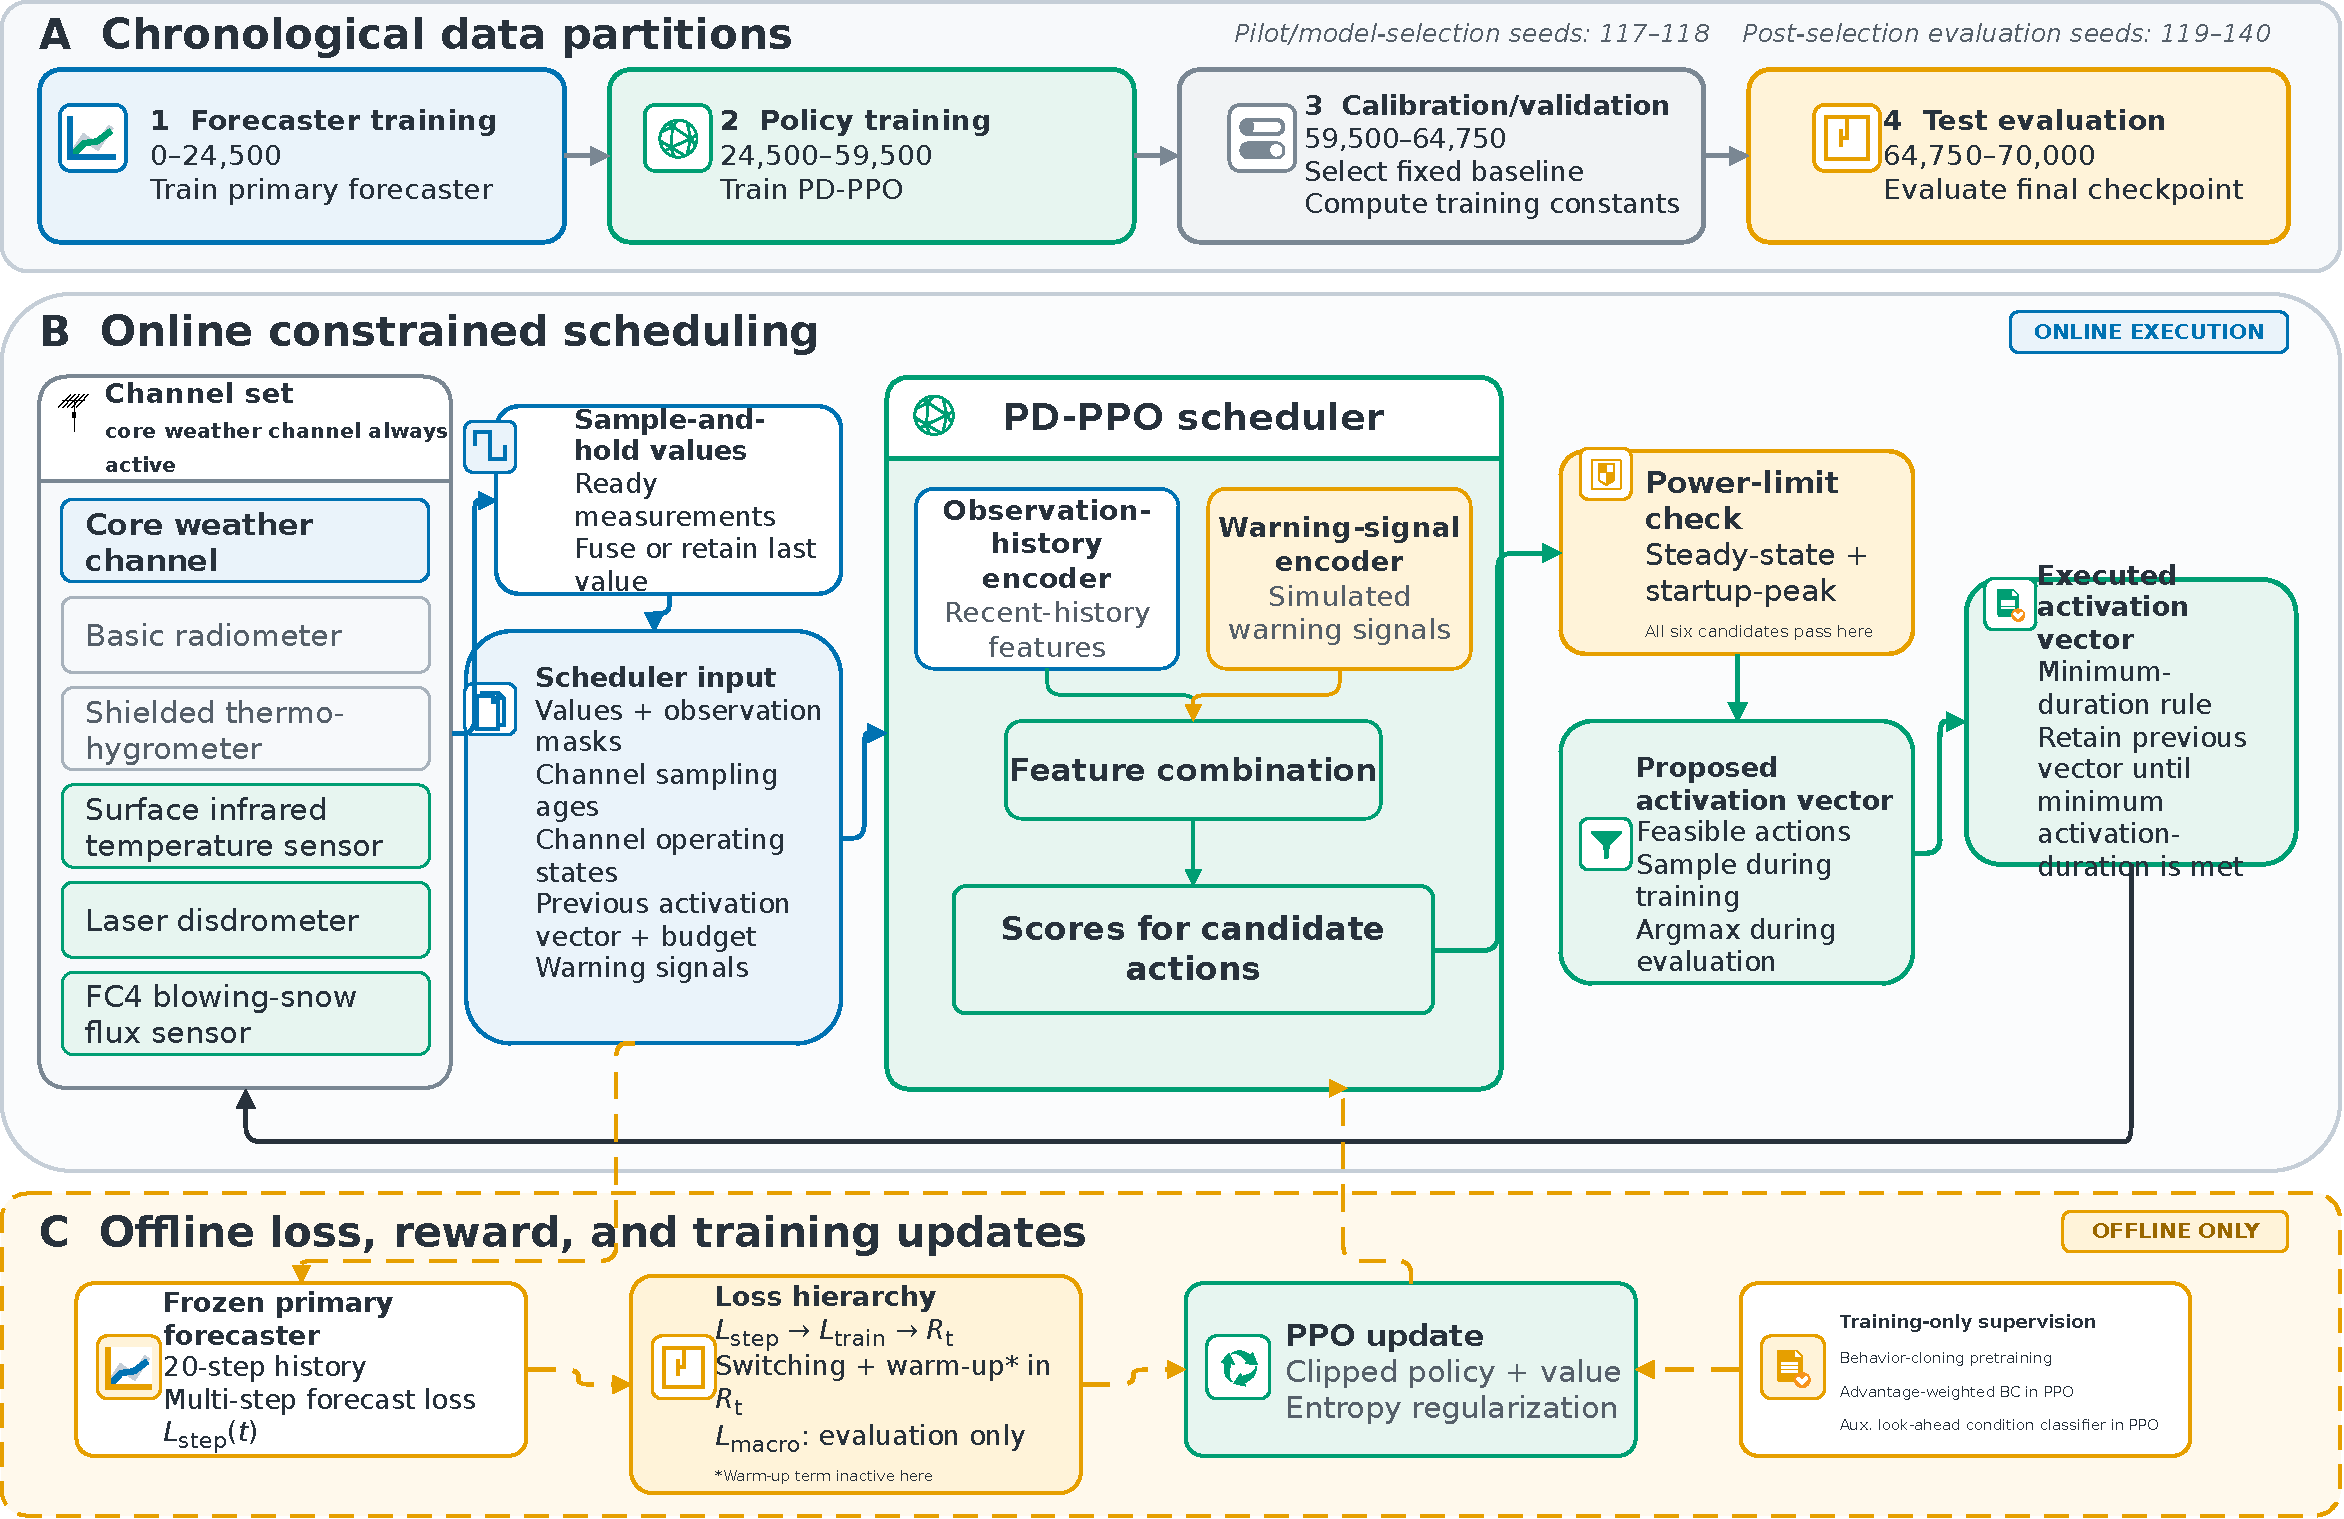
\includegraphics[width=\linewidth]{figure_pdppo_framework_drawio.pdf}
  \caption{Chronological data partitions and the PD-PPO scheduling loop. Panel A presents
  the forecaster-training, policy-training, calibration/validation, and test partitions in
  chronological order; training constants and the supervised-action mapping are
  determined from calibration/validation data before policy optimization.
  Panel B shows how the scheduler input is converted into a proposed channel
  subset and then into the executed subset under the feasibility and minimum
  dwell-time constraints. Panel C presents the frozen-primary-forecaster
  computation of forecast loss, its conversion to training loss and policy
  reward, and the PPO and supervised updates.}
  \label{fig:pdppo_framework}
\end{figure}

At each time step, the scheduler input includes recent sample-and-hold values
and observation masks together with channel-level runtime information. It also
includes the previously executed channel subset, budget and time features, and
simulated warning signals. The current condition label weights the training loss,
while a future-condition supervision label constructs the supervised target
action and trains the auxiliary future-condition classifier. Neither label is a
deployment-time scheduler input. During evaluation, current condition labels group the
reported results. The frozen primary forecaster remains fixed throughout policy
training and evaluation. The policy
selects a proposed channel subset, and the minimum dwell-time constraint
determines whether it can be executed or the previous subset must remain active.

The evaluation uses a controlled simulation of cold-region monitoring motivated
by Antarctic blowing-snow sensing. The six-channel system keeps the meteorological core
channel active and permits at most one of five optional channels to operate.
Candidate actions are checked against the power and startup constraints. In this
$q=1$ instantiation, every candidate action satisfies both limits, so the
optional-channel cardinality and minimum dwell-time constraints provide the active
restrictions. Particle, flux,
and thermal events favor different optional channels. The primary comparison uses
a fixed schedule selected on the calibration/validation partition; a warning-rule baseline
using the same deployment-available simulated warnings is the practical adaptive
comparator.

The primary analysis covers 22 post-selection evaluation seeds. Across these 22
seeds, the complete PD-PPO training configuration has lower macro-averaged
normalized forecast loss than the validation-selected fixed-schedule baseline in
every seed. The same configuration also has lower mean forecast loss than that
baseline in every seed, with reductions of 8.0\% and 10.6\%, respectively. Both
endpoints remain lower in every seed over the continuous 5,242-step scoreable test
partition. The PD-PPO scheduler also has lower losses than the AoI-priority,
round-robin, random-feasible, and privileged one-step look-ahead reference using
next-step test targets in every seed. Its macro-averaged loss is lower than that of
the Double DQN training configuration in all 22 seeds and lower than that of the
ridge-forecaster-selected fixed schedule in 21. A separate 24-seed descriptive aggregate retains
the two pilot/model-selection seeds and the previously reported 10.1\% and 7.9\%
reductions. The confidence intervals for comparisons with the two alternative
scalar-objective PPO training configurations and the warning-rule and privileged true-label baselines
include zero. The
true-label baseline uses current and future condition labels that are unavailable
during deployment, so it does not define an upper bound for feasible sequential
policies.

The study makes three contributions.
\begin{enumerate}[leftmargin=1.4em]
  \item The study formulates sensor scheduling under power constraints as a
  sequential decision problem. It gives sufficient conditions under which
  condition-dependent channel selection improves on fixed policies that always
  select one optional channel
  and shows that forecast loss, AoI, and objectives based on covariance trace can rank feasible
  schedules differently.

  \item The PD-PPO scheduler uses a complete training configuration that combines
  a forecast-loss policy reward, behavior cloning pretraining, continuing
  advantage-weighted behavior cloning during PPO, and auxiliary future-condition
  classification. A feasibility check enforces steady-state and startup power
  limits, and the minimum dwell-time constraint
  determines the executed subset.

  \item The evaluation compares matched PPO training configurations with forecast-loss,
  AoI, and bounded diagonal uncertainty-proxy objectives and includes a
  Double DQN training-configuration comparison. Action-sequence analysis examines
  policy behavior; full-partition and alternative-forecaster analyses assess
  sensitivity to temporal support and forecaster choice.
\end{enumerate}

\section{Background and Related Work}

\subsection{Resource-constrained sensing}

Resource-constrained sensor scheduling has been studied extensively in estimation,
communication, and energy-aware monitoring. Estimation-oriented formulations
minimize state-estimation error or posterior covariance
\citep{Shi_2011,AlAhdab2025}. Energy-harvesting censoring policies optimize the
utility of transmitted measurements \citep{FernandezBes2015}, while
freshness-driven policies use age of information (AoI) or age of incorrect
information \citep{Kaul_2012,Jonah2026}. Reinforcement learning has also been
applied to tracking and belief-state scheduling \citep{Qu2022,Alali2024} and to
delay-aware remote estimation with broader scheduling objectives
\citep{Tran2026}. These objectives directly match evaluation criteria based on
measurement freshness or current uncertainty. The present forecasting problem
retains the resource constraints and uses forecast loss as the scheduling
objective. A channel receives greater scheduling value when its observations
reduce forecast loss over the evaluation horizon.

A forecast-loss objective is particularly relevant for heterogeneous sensing
systems. A meteorological core channel can provide inexpensive and broadly useful
measurements, while optional channels may provide their greatest forecasting
benefit near specific physical events. The validation-selected fixed-schedule
baseline therefore provides a meaningful comparator. The evaluation compares observation-dependent
scheduling with fixed and dynamic baselines and with a privileged true-label baseline.

\begin{table}[htbp]
  \centering
  \caption{Position of this work relative to nearby scheduling and sensing literatures.}
  \label{tab:related_work_positioning}
  \footnotesize
  \setlength{\tabcolsep}{3.0pt}
  \renewcommand{\arraystretch}{0.96}
  \begin{tabular}{@{}>{\raggedright\arraybackslash}p{0.23\linewidth}>{\raggedright\arraybackslash}p{0.25\linewidth}>{\raggedright\arraybackslash}p{0.22\linewidth}>{\raggedright\arraybackslash}p{0.20\linewidth}@{}}
    \toprule
    Literature line & Typical optimization target & Scheduling structure & What this paper adds \\
    \midrule
    State-estimation and AoI scheduling
      & Covariance, estimation error, information age
      & Sensor selection under communication or energy limits
      & Multi-step forecast loss is the objective. \\
    Active perception and adaptive observation selection
      & Task information under partial observability
      & Observation actions selected from partial observations
      & A mandatory meteorological core channel, limited optional-channel capacity,
        and baselines that use information unavailable during deployment. \\
    DRL-based adaptive sensing and sensor steering
      & Information gain, coverage, data acquisition utility, or monitoring reward
      & Learned adaptive policies, often with soft or task-specific constraints
      & A finite candidate action set enforces the mandatory-core and
        optional-channel-capacity rules, and a feasible-action mask checks the
        steady-state and startup-peak power limits. \\
    Time series forecasting models
      & Forecast accuracy after the observation stream is given
      & Forecasting model for a given observation stream
      & A frozen primary forecaster evaluates every schedule; its parameters are fixed during policy training and evaluation. \\
    \bottomrule
  \end{tabular}
\end{table}


\subsection{Adaptive sensing and learning-based scheduling}

Forecast-oriented sensor scheduling is related to active perception and partially
observable decision making. In these settings, an agent selects observations
sequentially to improve a downstream task
\citep{Bajcsy2018,Lauri_2023}. Related theoretical work studies adaptive
observation selection under partial observability \citep{Golovin2011}. These
formulations support policies that respond to available observations. They do not
address how forecast-oriented channel selections should be executed under
steady-state power limits, startup-peak power limits, and a minimum dwell-time
constraint.

Deep reinforcement learning has been used for resource-constrained adaptive
sensing and sensor steering \citep{Murad2020,Ogbodo2025}, informative path
planning \citep{Wei2020}, and constrained optimization with delayed rewards
\citep{Pendyala2024}. Its sequential objective can account for consequences that
emerge over multiple time steps. Explicit feasibility enforcement is required when
the sensing system cannot execute arbitrary actions. The PD-PPO policy is
categorical over candidate action indices, and the scheduler applies a
feasible-action mask at each time step. The mask removes indices whose candidate
activation vectors violate the steady-state or startup-peak power limit.

\subsection{Forecasting models for schedule evaluation}

Forecasting models can quantify the downstream prediction loss associated with
an observation sequence produced by a sensor schedule. Relevant architectures
include the Temporal Fusion Transformer, temporal convolutional networks, and
iTransformer \citep{Lim2021,Bai2018,Liu2024}. The primary forecaster is trained
on the forecaster-training partition, and its parameters are held fixed throughout
policy training and evaluation. During policy training, it provides the
multi-step forecast-loss term used to construct the policy reward. During test
evaluation, it measures the forecast loss of the observation sequence produced
by each schedule. The alternative-forecaster analysis applies a ridge forecaster
to the same observation sequences and reselects the fixed-schedule baseline on the
calibration/validation partition. This sensitivity analysis quantifies the same
comparison under a second forecasting model.

\subsection{Antarctic blowing-snow monitoring}

Antarctic automatic weather station (AWS) networks and blowing-snow monitoring
provide the application context for the simulation. Antarctic AWS networks supply long-term
atmospheric and surface observations, while their spatial instrument coverage
remains uneven \citep{AntAWS2023}. Field measurements and numerical models
have been used to study drifting-snow occurrence and transport,
atmosphere--snow interactions, and snow particle properties
\citep{Amory2020,Sharma2023,Monrad2026}. The controlled simulation represents
this setting with one mandatory meteorological core channel and five optional channels.
At most one optional channel can operate at a time. For each seed, the PD-PPO scheduler and all
baselines are evaluated on the same simulated ground-truth time series.

\section{Problem Formulation}

\subsection{Sensor scheduling formulation}

Let $x_t \in \mathbb{R}^d$ denote the simulated physical state at time step
$t$. The state contains meteorological and blowing-snow variables, including
wind speed and direction, air temperature, relative humidity, air pressure,
solar radiation, snow surface temperature, snow particle statistics, and snow mass flux. Let
$a_t \in \{0,1\}^m$ denote the activation vector applied to the $m$ logical
channels at time step $t$. Each logical sensing channel is a simulation-level
unit with associated observations, power demand, startup demand, and warm-up
behavior.

\begin{table}[htbp]
  \centering
  \caption{Notation used for scheduler inputs, actions, and constraints.}
  \label{tab:notation_summary}
  \footnotesize
  \setlength{\tabcolsep}{4pt}
  \begin{tabular}{@{}p{0.18\linewidth}p{0.72\linewidth}@{}}
    \toprule
    Symbol & Meaning \\
    \midrule
    $x_t$ & Simulated physical state at time step $t$ \\
    $o_t$ & Scheduler observation built from observation histories, channel modes, channel sampling ages, the previous executed activation vector, budget/time features, and simulated warning signals \\
    $\mathcal{A}$ & Candidate action set satisfying the core-channel and optional-channel capacity rules \\
    $K$ & Number of candidate activation vectors in $\mathcal{A}$ \\
    $n_{\mathrm{opt}}$ & Number of optional channels, $|\mathcal{S}|$ \\
    $\mathcal{F}_t$ & Feasible activation-vector set satisfying the steady-state and startup-peak power limits at time step $t$ \\
    $r_t$ & Remaining required activation time for the previous executed activation vector \\
    $a^{(k)}$ & Candidate activation vector indexed by $k$ \\
    $\mathcal{I}_t$ & Feasible action indices $\{k:a^{(k)}\in\mathcal{F}_t\}$ \\
    $u_t$ & Proposed action index sampled or selected from $\mathcal{I}_t$ \\
    $\bar a_t=a^{(u_t)}$ & Proposed activation vector \\
    $a_t$ & Executed activation vector after the minimum dwell-time constraint \\
    \bottomrule
  \end{tabular}
\end{table}

\begin{table}[htbp]
  \centering
  \caption{Notation used for forecast losses, supervision, and policy training.}
  \label{tab:notation_objectives}
  \scriptsize
  \setlength{\tabcolsep}{4pt}
  \begin{tabular}{@{}p{0.18\linewidth}p{0.72\linewidth}@{}}
    \toprule
    Symbol & Meaning \\
    \midrule
    $L_{\mathrm{step}}$ & Per-step multi-step forecast loss with component-wise clipping at 10 \\
    $L_{\mathrm{train}}$ & Condition-weighted, calibration/validation-normalized training loss used in the policy reward \\
    $L_c$ & Event-type-specific forecast loss for event type $c$ \\
    $s_c$ & Median calibration/validation event-type-specific forecast loss across candidate fixed channel subsets for $c\in\{\mathrm{particle},\mathrm{flux},\mathrm{thermal}\}$ \\
    $s_{\mathrm{calm}}$ & Median overall calibration/validation forecast loss across the same candidate fixed channel subsets; default normalization factor for calm time steps \\
    $L_{\mathrm{macro}}$ & Macro-averaged normalized forecast loss with equal weights for the three event types \\
    $L_{\rho}$ & Weighted normalized forecast loss used in Proposition~\ref{prop:specialist_bottleneck} \\
    $\mathcal{V}_{\mathrm{AoI}}$ & Observed variables whose ages enter the theoretical AoI objective; not necessarily the forecast-target set $\mathcal{Y}$ \\
    $\pi_{\text{label}}$ & Theoretical privileged policy with access to condition labels \\
    $\pi_s$ & Fixed-channel policy that selects optional channel $s$ \\
    $c_t$ & Current condition label used for training-loss weighting on the policy-training partition and offline loss computation and grouping on the test partition; never a policy or critic input at decision time \\
    $c_t^{\mathrm{sup}}$ & Future-condition supervision label: the first non-calm condition label in $[t,t+16]$, or calm if none occurs; used only for behavior cloning and auxiliary classification during policy training \\
    $\ell_t$ & Indicator of a valid supervised target action; $\ell_t=1$ at every PPO step in the reported stride-one configuration \\
    $\eta_t$ & Indicator of an available future-condition supervision label for the auxiliary classifier; $\eta_t=\ell_t=1$ at every PPO step in the reported stride-one configuration \\
    $S_t$ & Normalized Hamming distance $m^{-1}\lVert a_t-a_{t-1}\rVert_1$; fraction of executed channel activation bits that change \\
    $W_t$ & Number of warm-up interruptions at time step $t$ \\
    \bottomrule
  \end{tabular}
\end{table}


The sensing system contains a mandatory meteorological core channel and a set of
optional channels. The core channel remains active because it supplies the
minimum measurements needed by the downstream forecast task. At most one
optional channel can be active at each time step. The candidate action set is
\begin{equation}
  \mathcal{A}
  =
  \left\{a\in\{0,1\}^{m}\;\middle|\;
    a_{\mathrm{met}}=1,\;
    \sum_{i\in\mathcal{S}}a_i\leq1
  \right\}.
  \label{eq:candidate_action_set}
\end{equation}

Given the previously executed activation vector $a_{t-1}$, the feasible set
contains the candidate actions that satisfy the steady-state and startup-peak power
limits.
\begin{equation}
  \begin{aligned}
  \mathcal{F}_t
  =\bigg\{a\in\mathcal{A}\;\bigg|\;&
    \sum_i p_i a_i\leq B,\\[-2pt]
  & \sum_{i:a_{t-1,i}=1} p_i a_i
    +\sum_{i:a_{t-1,i}=0}
      \max\!\left(p_i,p_i^{\mathrm{peak}}\right)a_i
    \leq B^{\mathrm{peak}}
  \bigg\}.
  \label{eq:feasible_action_set}
  \end{aligned}
\end{equation}

Here, $\mathcal{S}$ denotes the optional-channel index set. The steady-state powers
$p_i$ and budget $B$ use a common normalized unit. The startup-peak powers
$p_i^{\mathrm{peak}}$ and budget $B^{\mathrm{peak}}$ use a second common
normalized unit. An active channel contributes its steady-state power to the
startup-power check. A newly activated channel contributes the larger of its
steady-state and startup-peak power. Together with \Cref{eq:candidate_action_set}, these constraints permit a fixed
schedule to select one optional channel while preventing more than one optional
channel from operating at the same time.

The finite candidate set is indexed as
$\{a^{(1)},\ldots,a^{(K)}\}=\mathcal{A}$. At time step $t$, the feasible
indices are
\[
  \mathcal{I}_t=\{k:a^{(k)}\in\mathcal{F}_t\}.
\]
During training, the policy samples an index from $\mathcal{I}_t$. During
evaluation, it selects the highest-scoring feasible index. Let $u_t$ denote the
resulting index and let $\bar a_t=a^{(u_t)}$ be the proposed activation vector.
Let $r_t$ denote the remaining required activation time for the previous
executed activation vector. The executed activation vector is
\begin{equation}
  a_t=
  \begin{cases}
    a_{t-1}, & r_t>0,\\
    \bar a_t, & r_t=0.
  \end{cases}
  \label{eq:minimum_activation_rule}
\end{equation}

The feasible-action mask restricts the policy distribution to
$\mathcal{I}_t$ and enforces the steady-state and startup-peak power limits. The
execution rule retains $a_{t-1}$ until its minimum dwell time has been
completed. Each executed activation vector therefore remains active for at least
$D_{\min}$ time steps.

\subsection{Conditions under which optional-channel adaptation reduces forecast loss}

The sensing configuration with a mandatory meteorological core channel and at most one
active optional channel is a special case of a broader capacity-constrained
scheduling problem. Let $n_{\mathrm{opt}}=|\mathcal{S}|$ denote the number of
optional channels, of which the scheduler may select at most
$q<n_{\mathrm{opt}}$ at each time step. For an operating
condition $c\in\mathcal{C}$, let
$S_c^\star\subseteq\mathcal{S}$ denote an optimal optional-channel subset, with
$|S_c^\star|\leq q$.

Let $\widetilde L_c(\pi)$ denote the normalized forecast loss of policy $\pi$
under condition $c$. The weighted normalized forecast loss is
\[
L_{\rho}(\pi)
=
\sum_{c\in\mathcal{C}}
\rho_c\widetilde L_c(\pi),
\qquad
\rho_c>0,
\qquad
\sum_{c\in\mathcal{C}}\rho_c=1.
\]
The empirical macro-averaged normalized forecast loss in
\Cref{eq:macro_loss} uses
$\widetilde L_c(\pi)=L_c(\pi)/s_c$ and assigns equal weight to the particle,
flux, and thermal event types.

Dynamic scheduling can reduce forecast loss when no fixed optional-channel
subset is optimal for every condition with positive evaluation weight. The
advantage requires positive excess forecast loss when a fixed subset is
mismatched to the operating condition. Predictive information in the scheduler
input can then support channel changes before or during a condition transition.
The following proposition gives a sufficient condition for this advantage.

\begin{proposition}[Dynamic value with one active optional channel]
\label{prop:specialist_bottleneck}
Consider a scheduling problem that permits at most one active optional channel.
All policies are subject to the same startup and minimum dwell-time
constraints. For any $s\in\mathcal{S}$, let $\pi_s$ denote the fixed-channel
policy that selects $s$ under every operating condition. Suppose that at least
two positive-weight conditions have different optimal optional channels. The
corresponding condition intervals are long enough for the theoretical privileged
policy $\pi_{\text{label}}$, which has condition-label access, to complete
feasible channel changes under the common
execution constraints.

Transition losses are included in the normalized condition-specific losses.
For every fixed policy $\pi_s$ and every condition $c$,
\[
\widetilde L_c(\pi_s)
\geq
\widetilde L_c(\pi_{\text{label}}).
\]
For each positive-weight condition whose optimal channel differs from $s$,
\[
\widetilde L_c(\pi_s)
-
\widetilde L_c(\pi_{\text{label}})
\geq
\Delta_c
>
0.
\]
Then every fixed policy $\pi_s$ that always selects one optional channel
$s\in\mathcal{S}$ satisfies
\[
L_\rho(\pi_s)
>
L_\rho(\pi_{\text{label}}).
\]
\end{proposition}

A proof is provided in \ref{apx:specialist_bottleneck_proof}, and
\Cref{fig:specialist_bottleneck} illustrates the sufficient condition. The
proposition assumes that all policies follow the same startup and minimum
dwell-time constraints. It does not provide a performance bound for the
PD-PPO scheduler or any other implemented policy. The empirical privileged true-label baseline in
Supplementary Table S11 is not assumed to implement the theoretical
policy $\pi_{\text{label}}$ or to attain the minimum forecast
loss.

\begin{figure}[H]
  \centering
  \resizebox{\linewidth}{!}{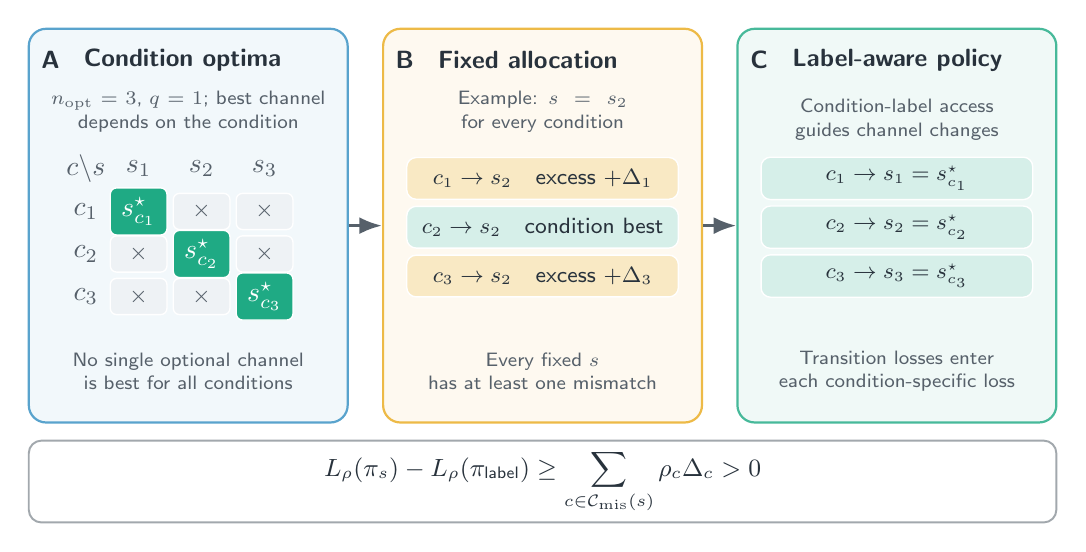
\begin{tikzpicture}[
  x=1cm,
  y=1cm,
  >=Latex,
  font=\sffamily\fontsize{7.8}{9.2}\selectfont,
  panel/.style={rounded corners=2.2mm,line width=0.8pt,minimum width=4.05cm,
    minimum height=5.00cm,inner sep=0pt},
  title/.style={font=\sffamily\fontsize{8.8}{10.3}\selectfont\bfseries,
    text=pdcharcoal,align=left},
  badge/.style={font=\sffamily\fontsize{9.2}{10.8}\selectfont\bfseries,
    text=pdcharcoal,align=center},
  subtitle/.style={font=\sffamily\fontsize{7.4}{8.6}\selectfont,
    text=pdslate,align=center,text width=3.65cm},
  matrixcell/.style={rounded corners=0.8mm,draw=white,line width=0.5pt,
    minimum width=0.72cm,minimum height=0.46cm,align=center},
  rowlabel/.style={font=\sffamily\bfseries,text=pdslate,align=right},
  item/.style={rounded corners=1.2mm,draw=white,line width=0.5pt,
    minimum width=3.45cm,minimum height=0.53cm,align=center},
  flow/.style={-Latex,line width=1.15pt,draw=pdslate},
  note/.style={font=\sffamily\fontsize{7.2}{8.5}\selectfont,text=pdslate,
    align=center,text width=3.65cm}
]
  \definecolor{pdblue}{HTML}{0072B2}
  \definecolor{pdteal}{HTML}{009E73}
  \definecolor{pdorange}{HTML}{E69F00}
  \definecolor{pdslate}{HTML}{56606A}
  \definecolor{pdcharcoal}{HTML}{28323C}
  \definecolor{pdlight}{HTML}{EEF2F5}

  \node[panel,fill=pdblue!5,draw=pdblue!65] (panelA) at (2.05,0) {};
  \node[panel,fill=pdorange!6,draw=pdorange!72] (panelB) at (6.55,0) {};
  \node[panel,fill=pdteal!6,draw=pdteal!72] (panelC) at (11.05,0) {};

  \node[badge] at (0.30,2.10) {A};
  \node[title,anchor=west] at (0.60,2.10) {Condition optima};
  \node[subtitle] at (2.05,1.45)
    {$n_{\mathrm{opt}}=3$, $q=1$; best channel\\depends on the condition};
  \node[rowlabel] at (0.75,0.72) {$c\backslash s$};
  \node[rowlabel] at (0.75,0.18) {$c_1$};
  \node[rowlabel] at (0.75,-0.36) {$c_2$};
  \node[rowlabel] at (0.75,-0.90) {$c_3$};
  \node[rowlabel,align=center] at (1.42,0.72) {$s_1$};
  \node[rowlabel,align=center] at (2.22,0.72) {$s_2$};
  \node[rowlabel,align=center] at (3.02,0.72) {$s_3$};
  \node[matrixcell,fill=pdteal!88,text=white,font=\sffamily\bfseries]
    at (1.42,0.18) {$s_{c_1}^{\star}$};
  \node[matrixcell,fill=pdlight,text=pdslate] at (2.22,0.18) {$\times$};
  \node[matrixcell,fill=pdlight,text=pdslate] at (3.02,0.18) {$\times$};
  \node[matrixcell,fill=pdlight,text=pdslate] at (1.42,-0.36) {$\times$};
  \node[matrixcell,fill=pdteal!88,text=white,font=\sffamily\bfseries]
    at (2.22,-0.36) {$s_{c_2}^{\star}$};
  \node[matrixcell,fill=pdlight,text=pdslate] at (3.02,-0.36) {$\times$};
  \node[matrixcell,fill=pdlight,text=pdslate] at (1.42,-0.90) {$\times$};
  \node[matrixcell,fill=pdlight,text=pdslate] at (2.22,-0.90) {$\times$};
  \node[matrixcell,fill=pdteal!88,text=white,font=\sffamily\bfseries]
    at (3.02,-0.90) {$s_{c_3}^{\star}$};
  \node[note] at (2.05,-1.85)
    {No single optional channel\\is best for all conditions};

  \node[badge] at (4.80,2.10) {B};
  \node[title,anchor=west] at (5.10,2.10) {Fixed allocation};
  \node[subtitle] at (6.55,1.45) {Example: $s=s_2$\\for every condition};
  \node[item,fill=pdorange!23,text=pdcharcoal] at (6.55,0.60)
    {$c_1\rightarrow s_2$\quad excess $+\Delta_1$};
  \node[item,fill=pdteal!16,text=pdcharcoal] at (6.55,-0.02)
    {$c_2\rightarrow s_2$\quad condition best};
  \node[item,fill=pdorange!23,text=pdcharcoal] at (6.55,-0.64)
    {$c_3\rightarrow s_2$\quad excess $+\Delta_3$};
  \node[note] at (6.55,-1.85)
    {Every fixed $s$\\has at least one mismatch};

  \node[badge] at (9.30,2.10) {C};
  \node[title,anchor=west] at (9.60,2.10) {Label-aware policy};
  \node[subtitle] at (11.05,1.35) {Condition-label access\\guides channel changes};
  \node[item,fill=pdteal!16,text=pdcharcoal] at (11.05,0.60)
    {$c_1\rightarrow s_1=s_{c_1}^{\star}$};
  \node[item,fill=pdteal!16,text=pdcharcoal] at (11.05,-0.02)
    {$c_2\rightarrow s_2=s_{c_2}^{\star}$};
  \node[item,fill=pdteal!16,text=pdcharcoal] at (11.05,-0.64)
    {$c_3\rightarrow s_3=s_{c_3}^{\star}$};
  \node[note] at (11.05,-1.85)
    {Transition losses enter\\each condition-specific loss};

  \draw[flow] (panelA.east) -- (panelB.west);
  \draw[flow] (panelB.east) -- (panelC.west);

  \node[rounded corners=1.6mm,draw=pdslate!55,fill=white,line width=0.7pt,
    minimum width=13.05cm,minimum height=0.78cm,align=center,
    font=\sffamily\fontsize{9.0}{10.6}\selectfont,text=pdcharcoal]
    at (6.55,-3.25)
    {$\displaystyle
      L_{\rho}(\pi_s)-
      L_{\rho}(\pi_{\text{label}})
      \geq \sum_{c\in\mathcal{C}_{\mathrm{mis}}(s)}
      \rho_c\Delta_c > 0$};
\end{tikzpicture}
}
  \caption{Sufficient condition for the value of adaptive scheduling with one
  active optional channel. Different operating conditions favor different
  optional channels, which causes every fixed policy that always selects one
  optional channel to incur excess
  loss for at least one condition. The theoretical privileged policy can change channels
  when the startup and minimum dwell-time constraints allow a feasible
  transition. The lower panel gives the resulting bound on weighted normalized
  forecast loss. The set $\mathcal{C}_{\mathrm{mis}}(s)$ contains the
  positive-weight conditions whose optimal channel differs from fixed channel
  $s$. The quantity $\Delta_c$ is the corresponding normalized excess loss.}
  \label{fig:specialist_bottleneck}
\end{figure}

\paragraph{Relation between the simulation and the proposition}
The simulation was designed to instantiate condition-dependent channel optima
of the type considered in \Cref{prop:specialist_bottleneck}. During particle,
flux, and thermal intervals,
the laser disdrometer channel, FC4 snow mass-flux channel, and infrared
snow-surface-temperature channel, respectively, provide the most reliable measurements of the
target variables emphasized for the corresponding event type. The event-type
decomposition on the test partition in
\Cref{tab:clean_regime_decomposition} evaluates whether the PD-PPO scheduler
reduces loss under these event-specific measurement requirements and improves
the macro-averaged normalized forecast loss. It does not verify the proposition's
inequality for every $\pi_s$ and the theoretical $\pi_{\mathrm{label}}$ in every
condition. The proposition does not require every event type to have lower loss
in every seed.

\subsection{Forecast loss and macro-averaged evaluation across event types}

The frozen primary forecaster receives a window of sample-and-hold values and
observation masks and predicts selected target variables at horizons
$k=1,\ldots,H$. Let $\hat{y}_{t+k,j}$ and $y_{t+k,j}$ denote the prediction
and target, respectively, for variable $j\in\mathcal{Y}$ at horizon $k$. The
condition label at time step $t$ is
\begin{equation}
  c_t\in\{\text{calm},\text{particle},\text{flux},\text{thermal}\}.
\end{equation}

Let $w_k$ denote the horizon weight, $\alpha_{j,c_t}$ the condition-specific
target weight, and $\sigma_j$ the scale of target variable $j$. The per-step
forecast loss is
\begin{equation}
  L_{\text{step}}(t)
  =
  \frac{
  \sum_{k=1}^{H}\sum_{j \in \mathcal{Y}}
  w_k \alpha_{j,c_t}
  \min\!\left\{10,\,
  \left| \hat{y}_{t+k,j} - y_{t+k,j} \right|/\sigma_j\right\}
  }{
  \sum_{k=1}^{H}\sum_{j \in \mathcal{Y}}
  w_k \alpha_{j,c_t}
  } .
  \label{eq:step_forecast_loss}
\end{equation}

The target scales satisfy $\sigma_j>0$, and all horizon and target weights are
nonnegative. The denominator is positive for every scoreable time step. Each
scale-normalized absolute error is capped at 10 before weighting and aggregation.

The experiment uses uniform horizon weights and the predeclared
condition-specific target weights in Supplementary Table S4. The condition
label determines which target weights are applied during policy training and
evaluation. It is not included in the scheduler input. Losses for PD-PPO and
all baselines are computed using the same target scales, target weights, and
condition labels.

An overall average can be influenced disproportionately by event frequency and
by differences in raw loss magnitude across event types. The macro-averaged normalized
forecast loss addresses these effects by normalizing each event-type-specific
loss with calibration/validation results from feasible fixed channel subsets and assigning
equal weight to the three event types. Let
$c\in\{\mathrm{particle},\mathrm{flux},\mathrm{thermal}\}$ index the event
types, and let $\mathcal{T}_c$ denote the evaluated test time steps labeled as
$c$. For a policy $\pi$, the event-type-specific forecast loss is
\begin{equation}
  L_c(\pi)
  =
  \frac{1}{|\mathcal{T}_c|}
  \sum_{t\in\mathcal{T}_c}
  L_{\text{step}}(t;\pi).
\end{equation}

For each event type $c$, the normalization factor $s_c$ is the median
event-type-specific forecast loss across the feasible fixed channel subsets
evaluated on the calibration/validation partition. The macro-averaged normalized forecast
loss is
\begin{equation}
  L_{\text{macro}}(\pi)
  =
  \frac{1}{3}
  \sum_{c\in\{\mathrm{particle},\mathrm{flux},\mathrm{thermal}\}}
  \frac{L_c(\pi)}{s_c}.
  \label{eq:macro_loss}
\end{equation}

This metric is reported when $|\mathcal{T}_c|>0$ and $s_c>0$ for all three
event types. Lower values indicate better forecasting performance. The metric
compares policies across equally weighted event types after accounting for the
median calibration/validation loss of feasible fixed channel subsets.

\subsection{Non-equivalence of forecast loss, AoI, and covariance objectives}

Forecast loss, AoI, and covariance trace evaluate different properties of a
sensor schedule. Let $\pi$ be a feasible scheduling policy and let
$\gamma\in(0,1]$ denote a discount factor. The same horizon $T$ and temporal
weights $\gamma^t$ are used for all three objectives. The discounted forecast objective is
\begin{equation}
  J_{\mathrm{fcst}}(\pi)
  =
  -\mathbb{E}_{\pi}
  \left[
    \sum_{t=0}^{T-1}\gamma^t
    L_{\mathrm{step}}(t;\pi)
  \right].
  \label{eq:forecast_objective}
\end{equation}

For a separate model-based estimator with posterior covariance $P_t$, let
$\mathcal{V}_{\mathrm{AoI}}$ denote the observed variables whose ages enter an
AoI objective. This set need not equal the forecast-target set $\mathcal{Y}$.
The AoI and covariance objectives are
\begin{equation}
  J_{\mathrm{AoI}}(\pi)
  =
  -\mathbb{E}_{\pi}\!\left[
    \sum_{t=0}^{T-1}\gamma^t
    \sum_{j\in\mathcal{V}_{\mathrm{AoI}}}\mathrm{age}_{t,j}
  \right],
  \qquad
  J_{\mathrm{cov}}(\pi)
  =
  -\mathbb{E}_{\pi}\!\left[
    \sum_{t=0}^{T-1}\gamma^t
    \mathrm{tr}(P_t)
  \right].
\end{equation}

The three objectives can induce different orderings over the same feasible
schedules. Such a difference can occur when sensor variables have unequal
downstream forecast value, even if one schedule produces fresher observations
and a lower estimator covariance.

\begin{proposition}[Non-equivalence of forecast loss, AoI, and covariance objectives]
\label{prop:non_equivalence}
Forecast loss, covariance trace, and per-variable AoI objectives can induce
different orderings over feasible sensor schedules. In particular, there exist
a common horizon $T$, a common discount factor $\gamma$, and two feasible
policies $\pi_1$ and $\pi_2$ such that
\begin{equation}
  J_{\mathrm{AoI}}(\pi_1) > J_{\mathrm{AoI}}(\pi_2),
  \qquad
  J_{\mathrm{cov}}(\pi_1) > J_{\mathrm{cov}}(\pi_2),
\end{equation}
and
\begin{equation}
  J_{\mathrm{fcst}}(\pi_2) > J_{\mathrm{fcst}}(\pi_1).
\end{equation}
Equivalently, $\pi_1$ has lower AoI and lower covariance trace, and
$\pi_2$ has strictly lower forecast loss.
\end{proposition}

The proof in \ref{apx:non_equivalence_proof} takes the common horizon $T=1$
and considers a single-target, single-horizon special case of
\Cref{eq:step_forecast_loss}. A policy that refreshes the variable with greater
influence on the forecast target has strictly lower forecast loss in the
constructed example, while its total AoI and covariance trace are both higher.
This ordering shows that forecast loss must be evaluated directly when sensor
variables have unequal downstream forecast value.
The AoI-priority, round-robin, and random baselines provide non-learned dynamic
comparisons. The matched scalar-objective PPO configurations replace the scalar
scheduling objective while retaining the shared supervision and architecture.

The proposition establishes that the objectives can rank feasible schedules
differently. It does not determine the performance ordering of policies learned
from finite training data. The comparisons in
\Cref{sec:matched_controls,sec:objective_learner_controls} examine whether the
forecast-loss, AoI, and bounded diagonal uncertainty objectives produce
measurable differences under matched PPO configurations. The empirical uncertainty proxy is not the
posterior covariance trace used in the proposition.

\section{PD-PPO Scheduler and Evaluation Protocol}
\label{sec:framework_protocol}

\subsection{Scheduler inputs, actions, and constraints}

The PD-PPO policy is trained using the policy reward in
\Cref{eq:training_reward}, whose forecast-loss term is derived from the
multi-step forecast loss in \Cref{eq:step_forecast_loss}. The macro-averaged
normalized forecast loss in \Cref{eq:macro_loss} is used for
event-type-balanced evaluation and does not enter PPO training. At each time step,
the scheduler receives recent sample-and-hold values and observation masks,
together with the time since each channel's last sampling opportunity. Its input
also includes channel operating states, the previous executed activation vector,
budget and time features, and simulated warning signals.
The reported actor and critic do not receive the remaining activation time
$r_t$ explicitly; the environment enforces the lock after an action is proposed.

The finite candidate action set is listed in
\Cref{tab:action_space_instantiation}. A feasibility check removes actions that
violate either the steady-state or startup-peak power limit and thereby forms the
feasible-action mask. During training, the policy samples an index from the
feasible action-index set. During evaluation, it selects the highest-scoring
feasible index. The resulting index specifies the proposed activation vector.
The minimum dwell-time constraint in \Cref{eq:minimum_activation_rule} is then
applied to determine the executed activation vector. Unless stated otherwise,
all baselines use the same feasibility check and execution rule.

\Cref{tab:action_space_instantiation} gives the candidate channel subsets used
by PD-PPO and the constrained baselines. Every subset includes the meteorological core
channel, and each differs only in whether and which optional channel is active. The evaluated
configuration therefore keeps one meteorological core channel active and allows at
most one optional channel to operate.

\begin{table}[htbp]
  \centering
  \caption{Candidate action set with a mandatory meteorological core channel and an
  optional-channel capacity of one.}
  \label{tab:action_space_instantiation}
  \footnotesize
  \setlength{\tabcolsep}{3.0pt}
  \begin{tabular}{@{}c p{0.35\linewidth} c p{0.21\linewidth} c@{}}
    \toprule
    Action index & Candidate channel subset & Power & Interpretation & \shortstack{Fixed-baseline\\selections} \\
    \midrule
    0 & Meteorological core channel & 0.25 & Core channel only & 0 of 22 \\
    1 & Meteorological core + basic radiometer channels & 0.33 & Optional channel & 0 of 22 \\
    2 & Meteorological core + shielded temperature--humidity channels & 0.43 & Optional channel & 0 of 22 \\
    3 & Meteorological core + infrared snow-surface-temperature channels & 0.74 & Thermal specialist channel & 9 of 22 \\
    4 & Meteorological core + laser disdrometer channels & 0.74 & Particle specialist channel & 2 of 22 \\
    5 & Meteorological core + FC4 snow mass-flux channels & 0.74 & Flux specialist channel & 11 of 22 \\
    \bottomrule
  \end{tabular}
  \vspace{0.4ex}

  \noindent\footnotesize
  Every candidate channel subset includes the meteorological core channel. The final
  column reports fixed baselines selected on the calibration/validation partition for the 22
  post-selection evaluation seeds. The scheduling decision selects at most one
  optional channel; action 0 selects none.
\end{table}


In the reported $q=1$ instance, the largest candidate steady-state demand is
$0.74<B=0.75$, and the largest startup-peak demand is $0.92<B_{\mathrm{peak}}=0.95$.
Consequently, every one of the six candidate action indices belongs to
$\mathcal{I}_t$ at every evaluated time step: neither power inequality excludes
a candidate activation vector. The feasibility layer remains part of the method,
but the active experimental restrictions are the optional-channel cardinality
constraint and the minimum dwell-time constraint.

Let $r_t$ be the remaining required activation time immediately before the action
at time $t$. If $r_t>0$, the environment executes $a_t=a_{t-1}$ regardless of
the proposed $\bar a_t$. After execution, the update is
\begin{equation}
  r_{t+1}=
  \begin{cases}
    D_{\min}-1, & a_t\neq a_{t-1},\\
    \max(r_t-1,0), & a_t=a_{t-1}.
  \end{cases}
  \label{eq:activation_timer_update}
\end{equation}
The first execution time step is therefore included in the $D_{\min}$-step
minimum. The reported values are $D_{\min}=6$ and a maximum channel warm-up of
two time steps. A newly activated channel cannot be deactivated before warm-up
completes, so $W_t=0$ structurally in this experiment.

\subsection{Partial observations and scheduler input}
\label{sec:partial_observation_update}

The environment maintains sample-and-hold values without a model-based Kalman
state estimate. Let $y_{t,i,j}$ denote a valid measurement of variable $j$
provided by ready channel $i$ at time step $t$, and let $R_{i,j}$ denote the
configured measurement-noise variance. Define $\mathcal{O}_{t,j}$ as the set
of ready channels that provide a valid measurement of variable $j$ at time
step $t$. For a scalar variable observed by at least one ready channel, the
fused value is
\begin{equation}
  \widetilde{x}_{t,j}
  =
  \frac{\sum_{i\in\mathcal{O}_{t,j}}R_{i,j}^{-1}y_{t,i,j}}
       {\sum_{i\in\mathcal{O}_{t,j}}R_{i,j}^{-1}} .
  \label{eq:observation_fusion}
\end{equation}

Wind-direction measurements are fused using a weighted circular mean. If
$\mathcal{O}_{t,j}=\varnothing$, the environment retains the previous value,
$\widetilde{x}_{t,j}=\widetilde{x}_{t-1,j}$. An observation mask indicates
whether each variable received a valid measurement at time step $t$. The
scheduler and frozen primary forecaster receive the most recent 20 value vectors
together with their observation masks. These masks distinguish new measurements
from retained sample-and-hold values.

For scalar variables, \Cref{eq:observation_fusion} assumes conditionally
independent measurement errors with variances $R_{i,j}$. Under correlated
channel errors, the rule provides a precision-weighted approximation. Computing
the minimum-variance linear estimate would require the full measurement-error
covariance matrix. The weighted circular mean for wind direction is defined
separately from the scalar fusion rule.

At each time step, the environment first updates the channel operating states
and identifies the ready channels. Measurement attempts are then performed for
the ready channels. Valid measurements are fused into the current variable
values, and variables without a valid measurement retain their previous values.
The environment subsequently updates the observation masks and channel-level
sampling ages before constructing the scheduler input.

For each channel, the scheduler receives its off, warming, or ready state,
remaining warm-up time, and normalized sampling age. The sampling age measures
the time since the channel's last sampling opportunity. It resets when an active
channel becomes ready to sample, including cases in which the stochastic
measurement attempt produces no valid measurement. Variable-level AoI follows
a different reset condition and counts the time steps since the variable's most
recent valid observation. The scheduler input further includes the previously
executed channel subset, current power ratio, diurnal phase, and compact
recent-history features.

The main policy does not receive an estimated covariance matrix. Covariance
trace is used in \Cref{prop:non_equivalence} as an alternative scheduling
objective. A diagonal predict--update uncertainty proxy is used only by the
uncertainty-objective PPO configuration.

The scheduler receives ten additional features computed deterministically from
the most recent 16 sample-and-hold value vectors and observation masks. The
features summarize recent patterns associated with particle, flux, and thermal
conditions. They also capture temporal trends and recent observation coverage.
All ten features are derived solely from information available at decision
time. Their complete definitions and clipping rules are provided in
Supplementary Section S1.

Four simulated warning signals are also available to the scheduler at decision
time. They represent particle, flux, thermal, and aggregate warning information
and include simulated noise. Condition labels are excluded from the scheduler
input. They are used to construct supervised information during training and to
group results during evaluation. A learned gate conditioned on the aggregate
warning signal combines the outputs of two feature encoders. The fused
representation is then used to compute the candidate-action scores. The critic
is implemented with a separate network. Supplementary Sections S1 and S5
provide the complete warning-signal construction and policy equations.

\begin{algorithm}[htbp]
\caption{PD-PPO policy training}
\label{alg:pdppo_training}
\small
\begin{algorithmic}
\State Train the primary forecaster on the forecaster-training partition and
freeze its parameters.
\State Evaluate the candidate fixed channel subsets on the calibration/validation partition,
compute $s_{\mathrm{calm}}$ and the event-type-specific normalization factors
$s_c$, and define the condition-specific supervised target-action mapping.
\State Pretrain the policy for 10,000 behavior cloning steps using the
supervised target actions derived from future-condition supervision labels.
\For{each PPO rollout of $n_{\mathrm{steps}}$ policy-training time steps}
  \State Initialize or continue a rollout on the policy-training partition.
  \For{each time step $t$ in the rollout}
    \State Construct $o_t$ from the observation history, channel-level runtime
    features, the previous executed activation vector, budget/time features, and
    simulated warning signals.
    \State Apply the feasibility check to obtain $\mathcal{I}_t$.
    \State Sample
    $u_t\sim\pi_{\theta}(\cdot\mid o_t,\mathcal{I}_t)$ and set
    $\bar a_t=a^{(u_t)}$.
    \State Apply the minimum dwell-time constraint to obtain $a_t$.
    \State Advance the sensing environment with $a_t$ and update the observation history.
    \State Evaluate the updated history with the frozen primary forecaster and compute
    $R_t$ using \Cref{eq:training_reward}.
    \State Store the sampled proposed-action index $u_t$, its log probability,
    the reward produced after executing $a_t$, and the training-only supervision.
  \EndFor
  \State Update the policy and critic for $n_{\mathrm{epochs}}$ passes over the
  rollout using the combined objective in \Cref{eq:pdppo_loss}.
\EndFor
\State Save the final policy checkpoint after the prescribed PPO updates and
freeze it for test evaluation.
\end{algorithmic}
\end{algorithm}

The implementation samples the policy at every training time step, including
when $r_t>0$. If the lock overrides a proposal, the rollout buffer retains the
proposed index $u_t$ and $\log\pi_{\theta_{\mathrm{old}}}
(u_t\mid o_t,\mathcal{I}_t)$, whereas the environment transition, reward, and
generalized advantage estimate are generated after executing
$a_t=a_{t-1}$. The reported training protocol therefore uses proposed-action
credit during locked time steps rather than an executed-action PPO likelihood.
The logs do not retain the counterfactual proposals needed to estimate the
override rate. This convention does not change the test losses of the frozen
final policies, but those losses do not evaluate an executed-action PPO update.

\subsection{Frozen primary forecaster and policy reward}

The primary forecaster is trained before policy optimization. Its parameters are
then frozen during policy training and evaluation.
It receives the 20-step sample-and-hold value history and its observation masks.
The time since each channel's last sampling opportunity, runtime, warning
signals, and the recent-history features above are provided only to the
scheduler. During policy training, the frozen primary forecaster returns the multi-step
forecast loss for the observation sequence produced by the current schedule.
That forecast loss forms the training loss in
\Cref{eq:subtype_normalized_training_loss}; the training loss and operational
penalties form the policy reward in \Cref{eq:training_reward}. During test
evaluation, the same frozen primary forecaster evaluates the observations produced
by the PD-PPO scheduler and every baseline.

Supplementary Table S10 separates quantities available to the online scheduler
from condition labels and future values used as training-only or evaluation-only
information. This distinction separates the privileged true-label baseline from the
PD-PPO scheduler.

The policy reward is the negative of the training loss plus the two operational
penalties used in the reported experiment.
\begin{equation}
  R_t
  =
  -\left[
  L_{\mathrm{train}}(t)
  + \lambda_{\mathrm{sw}} S_t
  + \lambda_{\mathrm{warm}} W_t
  \right],
  \label{eq:training_reward}
\end{equation}
where $L_{\mathrm{train}}$ is the condition-weighted training loss normalized
using calibration/validation quantities, $S_t$ is the normalized switching cost,
and $W_t$ is the number
of warm-up interruptions introduced at time step $t$. With $m$ logical channels,
the executed-action switching cost is
\begin{equation}
  S_t=\frac{1}{m}\lVert a_t-a_{t-1}\rVert_1.
  \label{eq:normalized_switching_cost}
\end{equation}
This normalized Hamming distance is the fraction of executed activation bits that
change between consecutive time steps. It is not a count of channel-switch
events.
Power
and startup violations are excluded by $\mathcal{I}_t$, and the minimum
dwell-time constraint determines $a_t$; these constraints therefore do
not enter the reward as residual violation terms.
The reported evaluation separates mean forecast loss from the macro-averaged
normalized forecast loss in
\Cref{eq:step_forecast_loss,eq:macro_loss}.

The training loss uses a condition-specific training weight and a normalization
factor computed on the calibration/validation partition while retaining calm
time steps and all three event types:
\begin{equation}
  L_{\mathrm{train}}(t)
  =
  \omega_{c_t}
  \frac{L_{\mathrm{step}}(t)}{s_{c_t}},
  \label{eq:subtype_normalized_training_loss}
\end{equation}
where $L_{\mathrm{step}}(t)$ is the clipped, target-weighted, scale-normalized
multi-step forecast loss returned by the frozen primary forecaster for the
current observation history, and $\omega_c\geq0$ is a condition-specific
training weight. For each event type
$c\in\{\mathrm{particle},\mathrm{flux},\mathrm{thermal}\}$, $s_c>0$ is the
median event-type-specific forecast loss across candidate fixed channel subsets
on the calibration/validation partition. The default factor $s_{\mathrm{calm}}>0$ is the
median overall forecast loss across the same candidates on that partition; it is
used for calm time steps. Thus the denominator $s_{c_t}$ in
\Cref{eq:subtype_normalized_training_loss} equals $s_c$ when $c_t$ is event type
$c$ and $s_{\mathrm{calm}}$ when $c_t$ is calm. The particle, flux, and thermal weights are 1.55, 0.95,
and 1.65, while calm time steps use unit weight. These weights and normalization
factors are fixed before policy optimization and remain unchanged during policy
training and evaluation. The current simulator-derived operating-condition label $c_t$ is
never available to the policy or critic at decision time. On the policy-training
partition, it selects the condition-specific weight and normalization factor in
\Cref{eq:subtype_normalized_training_loss}. On the test partition, it is used only
for offline loss computation and grouped reporting. Test action selection requires
the simulated warning signals but neither $c_t$ nor a reward value.

Policy learning uses two additional supervised signals formed only during
training. Define the future-condition supervision label $c_t^{\mathrm{sup}}$ as the
first non-calm simulator-derived condition label in the window from $t$ through
$t+16$, or calm when that window contains no event. This label selects a
predefined feasible supervised target action. The meteorological core channel is paired with the
shielded temperature--humidity channel in calm periods, the laser disdrometer channel for particle
events, the FC4 snow mass-flux channel for flux events, and the infrared
snow-surface-temperature channel for thermal events. These target actions supply
behavior cloning labels, while $c_t^{\mathrm{sup}}$ supervises an auxiliary
four-class future-condition classifier. Both signals are
formed only on the policy-training partition. The policy and critic receive the
simulated warning signals during policy-training rollouts and test evaluation.
Neither $c_t$ nor $c_t^{\mathrm{sup}}$ is available to the policy or critic at
decision time. The target actions are first used for 10,000 steps of
behavior cloning pretraining.
During PPO, the advantage-weighted behavior cloning term in \Cref{eq:bc_loss}
and the auxiliary future-condition classification term in
\Cref{eq:event_aux_loss} remain active.

The primary forecaster uses a TCN-style residual temporal convolutional
architecture \citep{Bai2018}. The implementation has three levels, 64 channels
per level, kernel size 3, and dropout rate 0.05. It is
fitted on the forecaster-training partition before policy training. Input and
target scales are fitted before policy updates, and the architecture is held
fixed throughout policy training and evaluation. No forecaster weights are
updated after the forecaster-training partition ends.

The forecaster is trained on observation sequences produced by full observation,
fixed channel subsets, and dynamic baselines in the forecaster-training
partition. This mixture exposes the model to dense histories and partial
histories produced by different schedules before its parameters are fixed. It
contains no calibration/validation or test observations.
Rollout counts, reset conditions, and the complete
training protocol are reported in Supplementary Section S2.

\subsection{PPO objective}

Let $o_t$ denote the scheduler input, $u_t$ the selected action index,
$\bar a_t=a^{(u_t)}$ the proposed activation vector, $a_t$ the executed
activation vector, and $\hat{A}_t$ the advantage estimate. The policy defines a
categorical distribution over the feasible action set,
\begin{equation}
  \pi_{\theta}(u\mid o_t,\mathcal{I}_t)
  =
  \frac{\exp z_{\theta}(o_t,u)}
  {\sum_{v\in\mathcal{I}_t}\exp z_{\theta}(o_t,v)}
  \mathbf{1}\{u\in\mathcal{I}_t\},
  \label{eq:masked_policy}
\end{equation}
where $z_{\theta}(o_t,u)$ is the policy score for activation vector $a^{(u)}$ and
$\mathcal{I}_t$ is the power- and startup-feasible index set. The activation
vector containing only the mandatory meteorological core channel belongs to the
candidate action set and satisfies both limits, so
$\mathcal{I}_t$ is nonempty at every time step.
PPO updates this distribution with the clipped surrogate
\begin{equation}
  \mathcal{L}_{\mathrm{clip}}(\theta)
  =
  -\mathbb{E}_t
  \left[
  \min\left(
  \rho_t(\theta)\hat{A}_t,\,
  \operatorname{clip}\!\left(\rho_t(\theta),1-\epsilon,1+\epsilon\right)
  \hat{A}_t
  \right)
  \right],
  \label{eq:ppo_clip}
\end{equation}
where
\begin{equation}
  \rho_t(\theta)
  =
  \frac{\pi_{\theta}(u_t\mid o_t,\mathcal{I}_t)}
       {\pi_{\theta_{\mathrm{old}}}(u_t\mid o_t,\mathcal{I}_t)} .
\end{equation}
The reported PPO loss contains the PPO surrogate, value loss, entropy
regularization, and two auxiliary terms tied to the forecast training setup.
\begin{equation}
  \mathcal{L}_{\mathrm{PPO}}
  =
  \mathcal{L}_{\mathrm{clip}}
  + c_v\mathcal{L}_{V}
  - c_H\mathcal{H}\!\left(\pi_{\theta}(\cdot\mid o_t,\mathcal{I}_t)\right)
  + \beta_{\mathrm{BC}}\mathcal{L}_{\mathrm{BC}}
  + \beta_{\mathrm{cond}}\mathcal{L}_{\mathrm{cond}} .
  \label{eq:pdppo_loss}
\end{equation}
For labeled training examples, let $u_t^{\mathrm{target}}\in\mathcal{I}_t$
denote the feasible supervised target action described above. The
advantage-weighted behavior cloning term is
\begin{equation}
  \mathcal{L}_{\mathrm{BC}}
  =
  -
  \frac{
  \sum_t \ell_t[\hat{A}_t]_+\,\log
  \pi_{\theta}(u_t^{\mathrm{target}}\mid o_t,\mathcal{I}_t)
  }{
  \sum_t \ell_t[\hat{A}_t]_+ + \varepsilon
  },
  \label{eq:bc_loss}
\end{equation}
where $[x]_+=\max(x,0)$ and $\ell_t\in\{0,1\}$ marks examples with a valid
supervised target. Let $\eta_t\in\{0,1\}$ mark examples for which the
future-condition supervision label is available to the auxiliary classifier. An
auxiliary future-condition classification loss is applied to the auxiliary
future-condition classifier. Let
$h_t$ be the policy representation, $q_{\theta}(c\mid h_t)$ the auxiliary
probability of operating condition
$c\in\{\mathrm{calm},\mathrm{particle},\mathrm{flux},\mathrm{thermal}\}$, and
$c_t^{\mathrm{sup}}$ the future-condition supervision label used only during policy
training. The reported stride-one configuration constructs both supervised
targets from the same $c_t^{\mathrm{sup}}$ and sets
$\eta_t=\ell_t=1$ at every PPO step. The general
implementation constructs the indicators separately. The auxiliary future-condition classification loss is
\begin{equation}
  \mathcal{L}_{\mathrm{cond}}
  =
  -
  \frac{
  \sum_t \eta_t \log q_{\theta}(c_t^{\mathrm{sup}}\mid h_t)
  }{
  \sum_t \eta_t + \varepsilon
  } .
  \label{eq:event_aux_loss}
\end{equation}

Supplementary Table S1 lists the full protocol and training hyperparameters.
\subsection{Reward-function and algorithm comparisons}
\label{sec:matched_controls}

The AoI-objective and uncertainty-objective PPO configurations retain the same PPO
policy and critic architecture, scheduler input, candidate action set, feasibility check,
chronological partitions, condition-specific weights, supervised target actions
available only during training, and auxiliary future-condition classification loss, but
replace the scalar forecast-loss objective. The AoI-objective PPO variant averages normalized
observed-variable age over the observation history; the uncertainty-objective
configuration averages a bounded diagonal predict--update variance proxy. Their
recursions and bounds are given in
Supplementary Section S3.
Each scalar objective supplies the corresponding rollout reward, from which the
value targets and advantages are computed. Replacing it therefore changes the
PPO surrogate, critic target, and the positive-advantage weights in
$\mathcal{L}_{\mathrm{BC}}$. These are matched PPO training configurations with
different scalar objectives, not isolated scalar-reward ablations.

The Double DQN training configuration uses a dueling network and the same
feasible-action mask, state representation, reward, action set, constraints,
policy-training partition, and test windows as the PD-PPO scheduler. Online and
target networks implement the
Double DQN target over feasible next actions, with three-step returns and
experience replay. This configuration does not use behavior cloning pretraining, the continuing
advantage-weighted behavior cloning term, or the auxiliary future-condition
classifier. Its complete settings are listed in
Supplementary Table S1.

\subsection{Chronological data split and baselines}

Each simulated ground-truth time series is split into forecaster-training,
policy-training, calibration/validation, and test partitions. The
calibration/validation partition computes $s_c$ and $s_{\mathrm{calm}}$, defines
the condition-to-action mapping used to construct supervised targets on
policy-training data, and selects the fixed-schedule baseline. Test windows are
not used for forecaster training, policy updates,
supervised-target generation, fixed-baseline selection, or normalization-factor
fitting.

The calibration/validation interval follows the policy-training interval
chronologically. Computationally, however, its normalization factors,
condition-to-action mapping, and fixed-schedule selection are computed offline
before policy optimization and then held fixed. Calibration/validation
transitions are not used as policy-training rollouts.

The chronological split is summarized in Supplementary Fig. S1.

The fixed-schedule baseline tests whether adaptation is needed. The AoI-priority
baseline, round-robin baseline, and random-feasible baseline provide non-learned
dynamic comparisons under the same operating rules. The privileged one-step
look-ahead reference using next-step test targets chooses the currently best feasible action;
those targets are unavailable to the deployed scheduler. Its one-step objective omits
minimum dwell-time consequences, warm-up, and observation age. It therefore does not isolate the
value of sequential decision making. The warning-rule baseline maps simulated
warning signals to channel subsets selected on the calibration/validation
partition. The privileged true-label baseline receives the exact sequence
$c_t,\ldots,c_{t+16}$ at each decision; these condition labels are unavailable
to the deployed scheduler. Neither privileged baseline is a guaranteed upper
bound.

Supplementary Table S11 fixes the role of each baseline before the results
section.

Exact decision rules, calibration/validation choices, tie breaks, and information availability
for these baselines are listed in Supplementary Section S6.

\section{Simulation and Evaluation Setup}
\label{sec:simulation_setup}

\subsection{Simulated sensing system}

The evaluation uses a controlled simulation of a cold-region sensing system motivated by
Antarctic automatic weather stations (AWSs). The final experiment uses six
logical channels, consisting of one mandatory meteorological core channel and five
optional channels. \Cref{tab:sensor_specs} lists the channels and their normalized
scheduling costs. A platform rendering is retained in Supplementary Fig. S2 as
physical motivation, while the channel table defines
the logical-channel configuration evaluated in the experiments.

The simulation keeps the meteorological core channel active, and at most one optional
channel can be active. Core weather measurements remain available while the
optional-channel capacity is allocated among logical channels whose
forecast value changes across event types.

\begin{table}[htbp]
  \centering
  \caption{Logical channels and normalized scheduling costs.}
  \label{tab:sensor_specs}
  \small
  \setlength{\tabcolsep}{3.5pt}
  \begin{tabular}{@{}c >{\raggedright\arraybackslash}p{0.27\linewidth} >{\raggedright\arraybackslash}p{0.33\linewidth} c c c@{}}
    \toprule
    Idx & Logical channel & Main observed variables
        & $p_i$ & $p_i^{\mathrm{peak}}$ & Warm-up \\
    \midrule
    1 & Meteorological core channel
      & wind, air temperature, relative humidity, pressure
      & 0.25 & 0.30 & 0 \\
    2 & Basic radiometer channel
      & solar radiation
      & 0.08 & 0.10 & 0 \\
    3 & Shielded temperature--humidity channel
      & air temperature, relative humidity
      & 0.18 & 0.22 & 0 \\
    4 & Infrared snow-surface-temperature channel
      & snow surface temperature
      & 0.49 & 0.62 & 1 \\
    5 & Laser disdrometer channel
      & particle diameter, particle velocity, simulated particle latent variable
      & 0.49 & 0.62 & 2 \\
    6 & FC4 snow mass-flux channel
      & snow mass flux
      & 0.49 & 0.62 & 1 \\
    \bottomrule
  \end{tabular}
  \vspace{0.5ex}

  \noindent\footnotesize
  The meteorological core channel is mandatory. At each time step, the scheduler may
  activate at most one optional channel and may leave all optional channels
  inactive. The infrared snow-surface-temperature channel, laser disdrometer channel,
  and FC4 snow mass-flux channel are
  event-specific channels for thermal, particle, and flux event types,
  respectively; the basic radiometer channel and shielded temperature--humidity channel
  are additional optional channels. Condition labels are simulator-derived metadata
  used only for training, calibration/validation, or offline evaluation; they are not
  direct channel measurements.
\end{table}


\subsection{Simulated time-series generation}
\label{sec:simulator_construction}

Each seed generates a simulated ground-truth time series with wind, temperature,
humidity, pressure, radiation, snow-surface temperature, particle statistics, and
snow mass flux. The simulation model uses reference distributions from the Antarctic
AWS network and blowing-snow statistics. The meteorological variables are parameterized from the AntAWS
compilation \citep{AntAWS2023}. Event and particle ranges draw on numerical
modeling of atmosphere--snow interaction, Antarctic drifting-snow observations,
and cold-region particle measurements \citep{Amory2020,Sharma2023,Monrad2026}.
Blowing-snow events are produced by a semi-Markov process coupled to wind
exceedance.

The simulation contains particle, flux, and thermal event types. Each event type
changes a different part of the simulated physical state and is observed most
reliably by a different event-specific channel. The laser disdrometer is used for
particle events, the FC4 snow mass-flux channel for flux events, and the infrared
snow-surface-temperature channel for thermal events. Event balance, targets weighted by
event type, and the optional-channel capacity make all three event types matter
in the forecast loss. One fixed optional channel can be effective on average,
but no single optional channel covers the full
forecast objective.

The scheduler input also contains simulated warning signals for the three event
types. These noisy pre-onset signals are assumed available at decision time;
their construction and distinction from condition labels are specified in
Supplementary Section S5. They are simulator-generated and do not constitute a
validated field warning system.

Eight prespecified validation checks assess the simulated series, covering
meteorological structure and blowing-snow behavior \citep{Aloni2024}. They include wind
autocorrelation, event frequency, agreement between simulated and observed
distributions of scalar variables, event durations,
the flux--wind relationship, particle-size--wind correlation, and the wind-speed
power spectrum. All eight criteria pass their prespecified acceptance rules; the
full table and simulation-validation figure are
reported in \ref{apx:generator_validation}. These simulation validation checks document the
simulation construction and remain separate from test policy selection.

\subsection{Metrics, seeds, and statistical summaries}

The primary evaluation uses eight event-balanced evaluation windows of 512 time steps each.
A prespecified rule balances event types and emphasizes
transport periods. The rule
uses event coverage and transport intensity from the simulated ground-truth time series,
not any policy loss, and is applied identically to the PD-PPO scheduler and every baseline. Mean
forecast loss averages \Cref{eq:step_forecast_loss} over the resulting 4096
time steps. The two co-primary endpoints are mean forecast loss and the
macro-averaged normalized forecast loss in \Cref{eq:macro_loss}.
Normalization factors are computed from candidate fixed channel subsets on the
calibration/validation partition, so the loss is
specific to this simulation model. The primary forecaster architecture
and training setup are described in \Cref{sec:framework_protocol}.

Continuous full-partition evaluation examines performance beyond the event-balanced
windows. The same final policy checkpoints and the fixed channel subsets previously
selected on the calibration/validation partition start fresh continuous rollouts and are evaluated at every
test step with a complete eight-step future target. This gives 5,242 scoreable test time steps per seed, covering
$[64750,69992)$; only the last eight
time steps are excluded because their future targets are incomplete. The policies, fixed channel subsets, and normalization factors fitted on the calibration/validation partition are
unchanged, and no schedule is reselected from
this evaluation.

The primary analysis reports 22 post-selection evaluation seeds. Pilot/model-selection seeds 117 and 118 support
a prespecified two-variant architecture comparison using their selected
test-window metrics. The selected configuration is then held fixed for the 22
post-selection evaluation seeds (119--140).
For each seed, the same simulated ground-truth time series is used for the
PD-PPO scheduler, the fixed-schedule baseline,
AoI-priority, round-robin, and random schedules, and all reported baselines. The
validation-selected fixed-schedule baseline is listed before test
evaluation and then uses a constant feasible channel subset without fallback
rotations.

The two pilot/model-selection seeds were used for a prespecified comparison between the
reported warning-conditioned policy and a variant with an additional deterministic
feature encoder. The former was selected before the remaining seeds were run.
Across the 22 post-selection evaluation seeds (119--140), the complete PD-PPO training
configuration achieved lower macro-averaged normalized forecast loss than the
validation-selected fixed-schedule baseline in every seed (mean paired difference 0.0838;
95\% percentile bootstrap confidence interval for the mean paired difference
[0.0708, 0.0967]). The separate 24-seed descriptive aggregate retains the pilot
seeds. The simulation parameters, target weights, baseline
definitions, and reported training settings were held fixed for this expansion.

The main protocol hyperparameters are listed in Supplementary Table S1.
Fixed channel subsets and calibration/validation losses for each seed are listed in
Supplementary Table S9.

The alternative-forecaster analysis uses a ridge forecaster fitted on the same
forecaster-training partition for each seed. The ridge forecaster selects its own
fixed-schedule baseline using calibration/validation windows and then evaluates the unchanged
PD-PPO and fixed-baseline observation sequences. Within this analysis, no policy,
action sequence, or forecaster is updated from its test results. The current
operating-condition label $c_t$ is used offline to select the same
predeclared target weights for every baseline and groups the completed losses for the
macro-averaged normalized forecast loss.

Seed statistical summaries use paired differences because PD-PPO and each baseline
are evaluated on the same simulated ground-truth time series. For a
seed $s$, the paired difference is comparator loss minus PD-PPO loss; a positive
paired difference favors the PD-PPO scheduler. Alongside mean paired differences
and counts of seeds with lower loss, the results report medians and 95\%
percentile bootstrap confidence intervals for the mean paired difference over
seeds.

\subsection{Action-sequence analysis}

The analysis uses the concatenated executed-action sequences from the eight
event-balanced evaluation windows. It reports executed-action entropy,
consecutive-action-pair entropy, condition--executed-action mutual information,
mean normalized Hamming distance between adjacent executed masks, and optional-channel
activation frequency by operating condition. A sequence is classified as fixed-like when
one executed activation mask accounts for at least 95\% of actions and as simple-cycle-like
when the top three masks account for at least 85\% of actions and the best periodic match
up to lag 64 reaches 90\%. The complete behavior-complexity gate also evaluates the
unique executed-action count, both entropy diagnostics, and the predeclared
condition-dependence criteria. These diagnostics include the seven artificial boundaries
between independently reset windows. They support interpretation of the learned schedule; the primary performance
claim remains the paired forecast loss comparison.

\section{Results}
\label{sec:results}

The evaluation covers forecast accuracy and the executed schedules that produce
it. Mean forecast loss and macro-averaged normalized forecast loss are co-primary
endpoints. The validation-selected fixed-schedule baseline is the structural
primary comparator, and the warning-rule baseline is the practical adaptive
comparator. Scalar-objective and algorithm comparisons concern complete training
configurations rather than isolated components.

\subsection{Forecasting performance on event-balanced evaluation windows}
\label{sec:main_result}

\Cref{tab:clean_main_comparisons} reports the primary paired analysis for the 22
post-selection evaluation seeds (119--140). The complete PD-PPO training
configuration has lower mean forecast loss and lower
macro-averaged normalized forecast loss than the validation-selected
fixed-schedule baseline in all 22 seeds. Mean forecast
loss decreases from 1.5744 to 1.4073, a relative reduction of 10.6\%. The
macro-averaged loss decreases from 1.0440 to 0.9602, a relative reduction of
8.0\%. The mean paired differences against the fixed-schedule baseline are +0.1671 for
mean forecast loss and +0.0838 for the macro-averaged loss, with 95\%
percentile bootstrap confidence intervals for the mean paired differences that
remain above zero. The exact one-sided sign test probability for a direction
fixed as lower loss, conditional on 22 independent signs under a 0.5 null, is
$2.38\times10^{-7}$ for either co-primary endpoint.

Seeds 117 and 118 supplied selected test-window metrics for a two-variant pilot
architecture comparison, after which the selected configuration was frozen.
They are excluded from the primary analysis. Supplementary Table S12 retains the
24-seed descriptive aggregate, including the 10.1\% and 7.9\% reductions, without
assigning it post-selection inferential status.
The PD-PPO scheduler also has lower values of both losses than the AoI-priority,
round-robin, and random-feasible baselines in all 22 seeds.

\begin{table*}[htbp]
  \centering
  \caption{Baseline comparisons with the complete PD-PPO training configuration on the event-balanced evaluation windows over 22 post-selection evaluation seeds. A positive paired difference means that the baseline has higher loss than PD-PPO.}
  \label{tab:clean_main_comparisons}
  \footnotesize
  \setlength{\tabcolsep}{2.4pt}
  \begin{tabular}{@{}>{\raggedright\arraybackslash}p{0.22\textwidth}>{\raggedright\arraybackslash}p{0.36\textwidth}>{\raggedright\arraybackslash}p{0.36\textwidth}@{}}
    \toprule
    Baseline & \shortstack[l]{Mean forecast loss\\Seeds with lower loss;\\mean paired difference\\{[95\% bootstrap CI]}} & \shortstack[l]{Macro-averaged loss\\Seeds with lower loss;\\mean paired difference\\{[95\% bootstrap CI]}} \\
    \midrule
    Fixed-schedule baseline & 22 of 22; +0.1671 [+0.1231, +0.2164] & 22 of 22; +0.0838 [+0.0708, +0.0967] \\
    AoI-priority baseline & 22 of 22; +0.2619 [+0.2331, +0.2928] & 22 of 22; +0.1655 [+0.1430, +0.1898] \\
    Round-robin baseline & 22 of 22; +0.2571 [+0.2249, +0.2900] & 22 of 22; +0.1664 [+0.1427, +0.1917] \\
    Random-feasible baseline & 22 of 22; +0.2681 [+0.2366, +0.3019] & 22 of 22; +0.1684 [+0.1446, +0.1933] \\
    Privileged one-step look-ahead reference using next-step test targets & 22 of 22; +0.2746 [+0.2391, +0.3107] & 22 of 22; +0.1855 [+0.1559, +0.2173] \\
    Warning-rule baseline & 8 of 22; -0.0039 [-0.0102, +0.0019] & 9 of 22; +0.0011 [-0.0049, +0.0081] \\
    Privileged true-label baseline & 9 of 22; -0.0042 [-0.0108, +0.0011] & 10 of 22; +0.0017 [-0.0045, +0.0086] \\
    \bottomrule
  \end{tabular}
  \begin{minipage}{0.98\textwidth}
  \vspace{0.4ex}\footnotesize Each interval is a 95\% bootstrap confidence interval for the paired difference. The validation-selected fixed-schedule baseline is the structural primary comparator; the warning-rule baseline is the practical adaptive comparator. The one-step look-ahead reference uses next-step test targets, and the true-label baseline uses the exact sequence $c_t,\ldots,c_{t+16}$; both receive information unavailable during deployment, and neither is an upper bound. The warning-rule baseline uses the same simulator-generated warning signals available to PD-PPO and a mapping selected on the calibration/validation partition.
  \end{minipage}
\end{table*}


The eight separately reset 512-step windows are constructed from test truth to
balance particle, flux, and thermal coverage and emphasize transport intensity.
The resulting event-balanced evaluation windows do not represent the natural
test distribution.
Supplementary Table S7 tests whether that
sampling rule drives the result by evaluating the same final policy checkpoints
and the fixed channel subsets selected on the calibration/validation partition once
over all 5,242 scoreable test time steps in each continuous test partition. The
PD-PPO scheduler again has lower mean forecast loss and lower macro-averaged loss
in all 22 seeds. The mean paired differences are +0.1347 for mean forecast loss and +0.0836 for the
macro-averaged loss, and both 95\% percentile bootstrap confidence intervals for
the mean paired differences remain above zero. The
observed paired advantage therefore extends beyond the windows emphasizing transport periods
used for the primary balanced comparison.
\Cref{fig:clean_main_evidence} summarizes the seed-level paired differences for
the main comparison with the fixed-schedule baseline and the additional baselines.

\begin{figure}[htbp]
  \centering
  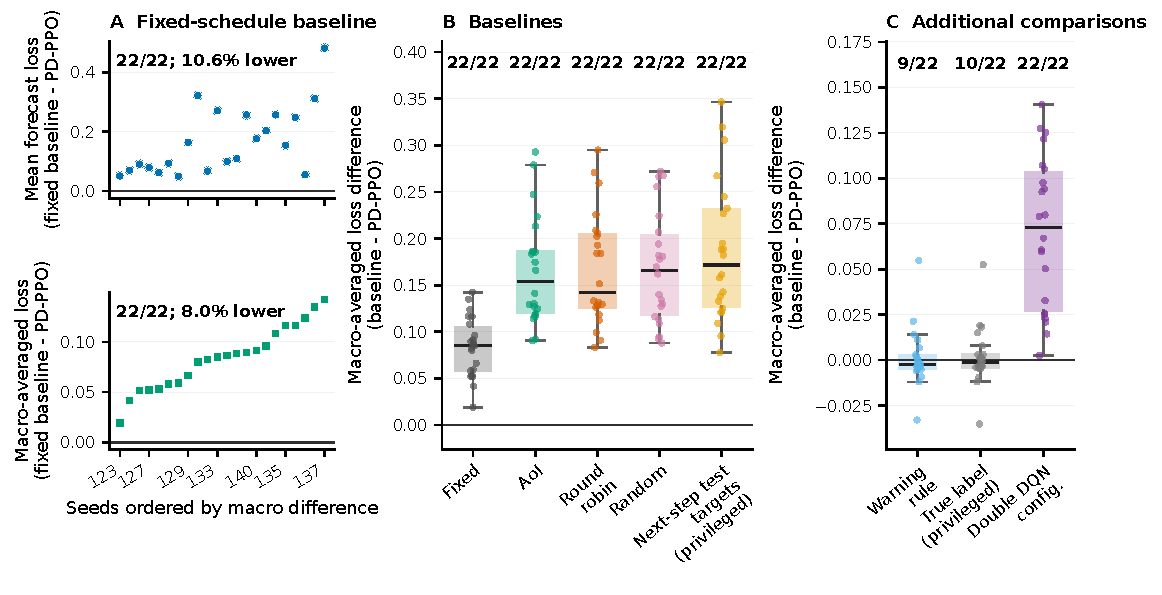
\includegraphics[width=\linewidth]{figure_clean_main_evidence.pdf}
  \caption{Seed-level paired differences over 22 post-selection evaluation seeds. Panel A
  compares PD-PPO with the fixed-schedule baseline. Panel B compares the
  AoI-priority, round-robin, and random-feasible baselines and the privileged
  one-step look-ahead reference using next-step test targets.
  Panel C compares the warning-rule and privileged true-label baselines and the Double DQN
  training configuration.
  Positive values mean that the baseline has higher loss than PD-PPO.}
  \label{fig:clean_main_evidence}
\end{figure}

\subsection{Channel activation across operating conditions}
\label{sec:regime_allocation}

The aggregate gain is distributed across all three forecast event types
(\Cref{tab:clean_regime_decomposition}). Mean paired differences are positive
for particle, flux, and thermal event types, and each 95\% percentile bootstrap
confidence interval for the mean paired difference remains above zero. The
PD-PPO scheduler has lower loss in 18 of 22 particle comparisons, 12 of 22
flux comparisons, and 15 of 22 thermal comparisons. Equal weighting combines
the three distinct specialist-channel requirements and yields lower
macro-averaged loss in all 22 seeds.

\begin{table}[htbp]
  \centering
  \caption{Event-type-specific forecast losses and the macro-averaged normalized forecast loss. Lower values are better; a positive paired difference favors PD-PPO over the fixed-schedule baseline.}
  \label{tab:clean_regime_decomposition}
  \scriptsize
  \setlength{\tabcolsep}{2.6pt}
  \begin{tabular}{@{}lcccc@{}}
    \toprule
    Event type & PD-PPO & Fixed baseline & \shortstack{Seeds with\\lower loss} & \shortstack{Mean paired difference\\{[95\% bootstrap CI]}} \\
    \midrule
    Particle event type & 1.0749 & 1.1037 & 18 of 22 & +0.0287 [+0.0148, +0.0473] \\
    Flux event type & 0.7639 & 0.8930 & 12 of 22 & +0.1291 [+0.0642, +0.1938] \\
    Thermal event type & 1.0418 & 1.1353 & 15 of 22 & +0.0935 [+0.0444, +0.1452] \\
    Macro-averaged loss & 0.9602 & 1.0440 & 22 of 22 & +0.0838 [+0.0708, +0.0967] \\
    \bottomrule
  \end{tabular}
\end{table}


\Cref{fig:clean_mechanism} compares optional-channel activation by PD-PPO and the
validation-selected fixed-schedule baseline. The laser disdrometer channel is active for
99.2\% of particle-event steps, the FC4 snow mass-flux channel for 97.8\% of
flux-event steps, and the infrared snow-surface-temperature channel for 99.7\% of
thermal-event steps. Calm periods use a mixture of the four optional channels with
nonzero test activation frequency. Calibration/validation selects the FC4 snow
mass-flux channel in 11 seeds, the infrared snow-surface-temperature channel in
nine, and the laser disdrometer channel in two, after which the selected subset
remains fixed on the test partition.

\begin{figure}[H]
  \centering
  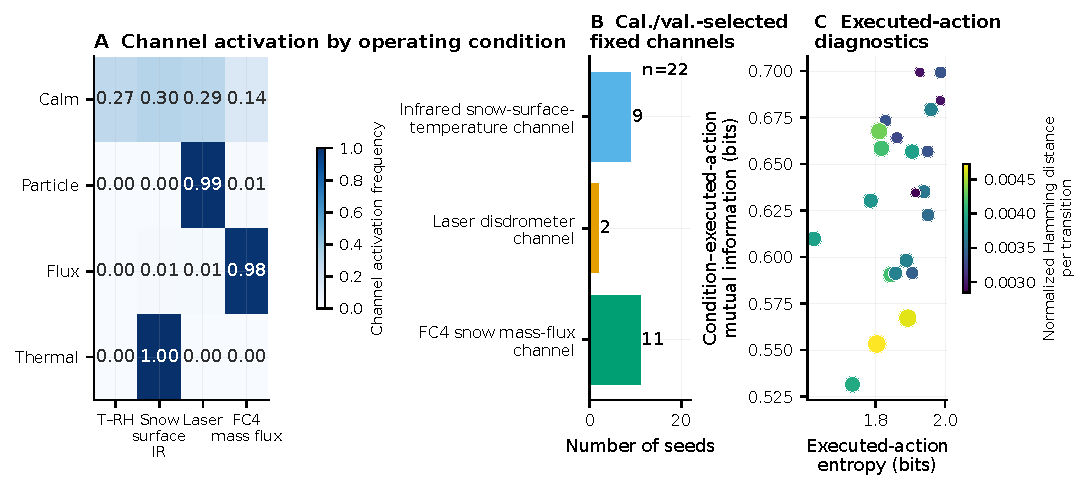
\includegraphics[width=\linewidth]{figure_clean_mechanism.pdf}
  \caption{Optional-channel activation by operating condition. Panel A shows the
  shielded temperature--humidity, infrared snow-surface-temperature, laser
  disdrometer, and FC4 snow mass-flux channels. Panel B shows the fixed channels
  selected on the calibration/validation partition. Panel C reports executed-action
  entropy, condition--executed-action mutual information, and mean normalized
  Hamming distance between adjacent executed masks.}
  \label{fig:clean_mechanism}
\end{figure}

All 22 executed-action sequences pass the behavior-complexity gate; none is
fixed-like or simple-cycle-like under its prespecified criteria. Mean
executed-action entropy is 1.872 bits, and mean condition--executed-action mutual
information is 0.632 bits. The mean normalized Hamming distance between adjacent
executed masks is 0.00369. The meteorological core channel remains active by
construction, while the executed schedules do not activate the basic radiometer
channel in the selected test windows. At least three of the four active optional
channels have intermediate channel activation frequency in every seed; all four
do so in 21 of 22 seeds.
No channel was deactivated before completing warm-up because $D_{\min}=6$
exceeds the maximum two-step warm-up. Executed channel changes occur mainly when
the operating condition changes.
The gate's fixed-like and simple-cycle-like criteria exclude fixed schedules and
simple cycles. These behavior diagnostics concatenate the
eight separately reset windows and include the seven reset boundaries; they are
descriptive diagnostics, not a primary performance endpoint.

\subsection{Scalar-objective and training-configuration comparisons}
\label{sec:objective_learner_controls}

The AoI-objective and uncertainty-objective PPO configurations retain the PPO
architecture, scheduler input, feasible-action mask, supervised target actions
used only during training, auxiliary future-condition classifier, chronological
partitions, and frozen primary forecaster, but use AoI or a bounded diagonal
uncertainty proxy as the scalar rollout objective. Because each objective supplies its own advantages,
the comparison also changes the PPO surrogate, value target, and
advantage-weighted behavior cloning weights. \Cref{tab:clean_learning_controls}
reports the paired differences from PD-PPO. The mean macro-averaged loss
difference is +0.0015 for the AoI configuration, with lower loss for the
forecast-loss-objective configuration in 12 of 22 seeds, and +0.0013 for the
uncertainty configuration, with lower loss in 12 of 22 seeds. For both
alternative configurations, both 95\% bootstrap confidence intervals for the
paired difference in macro-averaged loss and mean forecast loss include zero.
These comparisons establish neither a population-level directional difference
nor equivalence among scalar objectives. All three matched PPO configurations
nevertheless have lower macro-averaged loss than the fixed-schedule baseline in
all 22 seeds and meet the channel-use acceptance criterion in every seed.
Warm-up interruption is structurally zero for all
three configurations because $D_{\min}=6$ exceeds the maximum two-step warm-up.

The Double DQN training configuration uses the same scheduler observation,
reward based on forecast loss, action set, constraints, policy-training partition, and frozen primary
forecaster. PD-PPO has lower
macro-averaged loss in all 22 seeds and lower mean forecast loss in 21 of 22,
with mean baseline-minus-PD-PPO paired differences of +0.0706 and +0.1423,
respectively. Double DQN has lower macro-averaged loss than the fixed-schedule baseline
in 12 of 22 comparisons and meets the channel-use acceptance criterion
in 5 of 22 seeds; no channel can be deactivated before completing warm-up under
the reported $D_{\min}$. All test metrics use the same frozen primary forecaster.
This is a training-configuration comparison on the same scheduling problem,
because the complete PD-PPO configuration uses behavior cloning pretraining,
the continuing advantage-weighted behavior cloning term, and the auxiliary
future-condition classifier; it is not an isolated comparison of
the PPO and Double DQN update rules.

\begin{table*}[htbp]
  \centering
  \caption{Scalar-objective PPO and Double DQN training-configuration comparisons. A positive paired difference indicates lower loss for PD-PPO.}
  \label{tab:clean_learning_controls}
  \scriptsize
  \setlength{\tabcolsep}{2.1pt}
  \begin{tabular}{@{}>{\raggedright\arraybackslash}p{0.14\textwidth}>{\raggedright\arraybackslash}p{0.27\textwidth}>{\raggedright\arraybackslash}p{0.27\textwidth}>{\centering\arraybackslash}p{0.12\textwidth}>{\centering\arraybackslash}p{0.14\textwidth}@{}}
    \toprule
    Comparison & Mean forecast loss\newline Seeds with lower loss;\newline mean paired difference\newline [95\% bootstrap CI] & Macro-averaged loss\newline Seeds with lower loss;\newline mean paired difference\newline [95\% bootstrap CI] & Lower macro-averaged\newline loss than fixed baseline & Channel-use acceptance\newline criterion \\
    \midrule
    AoI-objective PPO configuration & 10 of 22; -0.0003 [-0.0073, +0.0063] & 12 of 22; +0.0015 [-0.0037, +0.0066] & 22 of 22 & 22 of 22 \\
    Uncertainty-objective PPO configuration & 10 of 22; +0.0008 [-0.0063, +0.0076] & 12 of 22; +0.0013 [-0.0035, +0.0054] & 22 of 22 & 22 of 22 \\
    Double DQN training configuration & 21 of 22; +0.1423 [+0.1036, +0.1827] & 22 of 22; +0.0706 [+0.0535, +0.0875] & 12 of 22 & 5 of 22 \\
    \bottomrule
  \end{tabular}
  \begin{minipage}{0.98\textwidth}
  \vspace{0.4ex}\footnotesize Each interval is a 95\% bootstrap confidence interval. The objective rows compare matched PPO training configurations with different scalar objectives. Each objective changes the PPO surrogate, value target, advantage, and the weights in the advantage-weighted behavior cloning term; the rows are therefore not isolated scalar-reward ablations. The configurations otherwise share the scheduler input, training-only supervised targets, auxiliary future-condition classifier, candidate action set, and constraints. The Double DQN row is a training-configuration comparison: it shares the state representation, reward based on forecast loss, action set, and constraints, but omits behavior cloning pretraining, the continuing behavior cloning term, and the auxiliary classifier. All configurations have zero warm-up interruption structurally because $D_{\min}=6$ exceeds the maximum two-step warm-up; the final column is therefore determined by the channel-use acceptance criterion. All test metrics use the same frozen primary forecaster.
  \end{minipage}
\end{table*}


\subsection{Baselines using additional information}
\label{sec:information_references}

The privileged one-step look-ahead reference using next-step test targets uses
information unavailable during deployment. At each time step it reads next-step targets on
the test partition and evaluates feasible actions with their next-step forecast
loss. Its one-step scoring does not account for the longer-term consequences of
the minimum dwell-time constraint, warm-up, and observation age. The PD-PPO scheduler
has lower mean forecast loss and lower macro-averaged normalized forecast loss
in all 22 seeds
(\Cref{tab:clean_main_comparisons}). For this reference, the mean normalized
Hamming distance between adjacent executed masks is 0.0280. Despite
access to next-step forecast loss, it has higher mean forecast loss and higher
macro-averaged normalized forecast loss in every seed, and its executed activation indicators change approximately 7.6 times as often as those of
PD-PPO.

The warning-rule baseline maps simulated warning signals to proposed actions.
The privileged true-label baseline uses the exact sequence $c_t,\ldots,c_{t+16}$
and a condition-to-action mapping selected on the calibration/validation
partition. These condition labels are unavailable during deployment.
Their mean macro-averaged loss differences from PD-PPO are
+0.0011 and +0.0017, respectively. For both baselines, the 95\% percentile
bootstrap confidence intervals for the mean paired differences include zero
for macro-averaged loss and mean forecast loss. These intervals establish neither
a population-level directional difference nor equivalence. The true-label baseline is neither
deployable nor an upper bound on feasible sequential control.

\subsection{Alternative-forecaster analysis}
\label{sec:secondary_forecaster}

The alternative-forecaster analysis evaluates the test observation sequences
with a ridge forecaster. Fixed-schedule selection was repeated on the
calibration/validation partition before test evaluation. PD-PPO has lower
macro-averaged loss than the primary-forecaster fixed-schedule baseline in all 22
comparisons and than the ridge-forecaster fixed-schedule baseline in 21 of 22
(Supplementary Table S8).
The mean paired difference against the fixed
schedule selected using the ridge forecaster is +0.1339,
with a 95\% percentile bootstrap confidence interval for the mean paired
difference of [+0.1103, +0.1563]. This evaluation changes both
the forecaster architecture and the validation-selected fixed-schedule baseline without retraining the
policy.
\Cref{fig:clean_controls} summarizes the scalar-objective comparisons and the two
ridge-forecaster comparisons.

\begin{figure}[H]
  \centering
  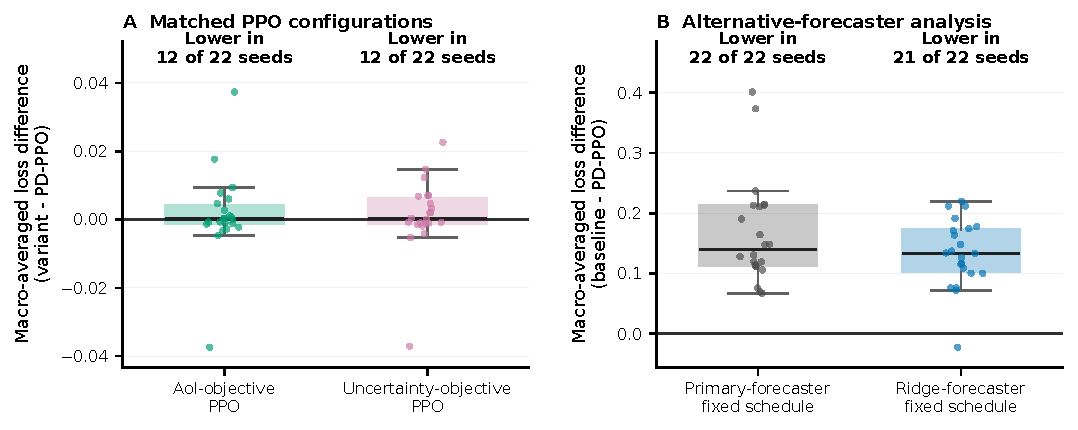
\includegraphics[width=\linewidth]{figure_clean_controls.pdf}
  \caption{Scalar-objective training-configuration comparisons and
  alternative-forecaster analysis over 22 post-selection seeds. Panel
  A compares matched PPO configurations with different scalar objectives. Panel B gives macro-averaged loss differences for the
  primary-forecaster fixed-schedule baseline and the fixed schedule selected with
  the ridge forecaster. Positive values mean that the baseline has higher loss than
  PD-PPO.}
  \label{fig:clean_controls}
\end{figure}

\section{Discussion}
\label{sec:discussion_future_work}

\subsection{Primary comparison with the fixed-schedule baseline}

Across the 22 post-selection evaluation seeds, the complete PD-PPO training
configuration achieved lower mean forecast loss and lower macro-averaged
normalized forecast loss than the validation-selected fixed-schedule baseline in
every seed. The separate 24-seed descriptive
aggregate, which includes two pilot/model-selection seeds, retains the same
direction. With the ridge forecaster, the paired difference against the fixed
baseline selected for that forecaster is positive in 21 of the 22 post-selection
seeds and 23 of 24 seeds in the descriptive aggregate. Evaluation over all
scoreable test steps also
retains lower values of both co-primary endpoints in every seed, so the observed
difference is not confined to the event-balanced evaluation windows.
Executed-action analysis shows that the scheduler activates the corresponding
specialist channel for each of the particle, flux, and thermal event types while
retaining a broader mixture during calm periods. This pattern was observed for
the complete training configuration, which includes simulated warning inputs and
future-condition supervision; it cannot be attributed to the scalar objective
alone.

The reported system has a mandatory meteorological core channel and an optional-channel
capacity of one. The underlying design problem extends to settings in which only
$q<n_{\mathrm{opt}}$ optional
channels can operate. In such systems, a scheduler must decide whether to
reserve the available capacity for one generally useful measurement or
reallocate it as forecast requirements change. The present $q=1$ optional-channel capacity makes that trade-off directly observable and
prevents simultaneous low-cost optional channels. The meteorological core channel
costs 0.25 normalized units and each event-specific channel costs 0.49. Although
two event-specific channels would exceed the 0.75 budget, such subsets are absent
from the candidate set. Every listed candidate has steady-state demand at most
0.74 and startup-peak demand at most 0.92, below the corresponding 0.75 and 0.95
limits. Both instantaneous power limits are enforced, but the feasible-action
mask therefore excludes no candidate in this instance. The empirical result is
established under the optional-channel cardinality constraint and minimum
dwell-time constraint, not under observed binding of the two power limits
(Supplementary Table S14).

\subsection{Condition-dependent activation relative to the fixed schedule}

Calibration/validation selects a strong fixed optional channel. The FC4 snow
mass-flux channel is selected in more than half of the seeds, and the infrared
snow-surface-temperature channel in most of the remainder. Such a schedule
avoids switching and can perform well when the evaluation distribution is
dominated by one measurement requirement. Its weakness appears when particle,
flux, and thermal event types all contribute to the forecasting objective. The
optional channel preferred for one event type is nearly absent from another, so
no single subset can preserve the three event-specific benefits. This pattern
instantiates the proposition's motivation, but the empirical table does not
verify all of its policy-by-condition assumptions.

The PD-PPO scheduler obtains the observed difference with sparse executed-action
changes. The mean normalized Hamming distance per transition is 0.00369,
consistent with the minimum dwell-time constraint and below the corresponding
rate for the one-step look-ahead reference under its one-step rule. Executed
changes mainly coincide with changes in operating condition, and no optional
channel dominates the sequence across event types. Nonzero
condition--executed-action mutual information and the behavior-complexity gate
distinguish these executed sequences from fixed-like or simple-cycle-like
schedules under the frozen thresholds. These quantities are descriptive and
include boundaries between the eight separately reset event-balanced evaluation
windows.

\subsection{Scalar-objective and training-configuration comparisons}

The matched AoI-objective and uncertainty-objective PPO configurations replace
forecast loss with AoI or a bounded diagonal uncertainty proxy while retaining
the shared PPO algorithm. \Cref{prop:non_equivalence} establishes a mathematical
distinction among the theoretical forecast-loss, AoI, and covariance-trace
objectives; the empirical uncertainty configuration uses a bounded diagonal
proxy rather than the full covariance trace. All three PPO configurations
receive the same condition-specific training weights, training-only supervised
target actions, and auxiliary future-condition classification labels. Each
scalar objective also changes the value target, advantage, PPO surrogate, and
advantage weights used in the continuing behavior cloning term. The feasible
action set is small, and four optional-channel choices have nonzero activation
frequency under the main policy. The 95\% percentile bootstrap confidence
intervals for the mean paired differences include zero for both matched
scalar-objective PPO configurations. These comparisons concern matched PPO
training configurations with different scalar objectives; they are not
reward-only ablations.

The Double DQN training configuration uses the same scheduler observation,
reward based on forecast loss, action set, and constraints. It has higher
macro-averaged loss in all 22 post-selection seeds and higher
mean forecast loss in 21 of 22 seeds than PD-PPO. Under the channel-use
acceptance criterion, Double DQN meets the criterion in 5 of 22 seeds;
no channel is deactivated before warm-up completes, as structurally required by
$D_{\min}=6$. The PD-PPO configuration also
contains behavior cloning pretraining, continuing advantage-weighted behavior
cloning, and an auxiliary future-condition classifier. The comparison therefore
concerns complete training configurations and does not establish a general
advantage of policy-gradient learning over value-based learning.

The privileged one-step look-ahead reference using next-step test targets can
inspect next-step forecast loss on the test partition and therefore has more
information per decision than the deployed scheduler. It still has higher loss
in every seed and a mean normalized Hamming distance about 7.6 times as large.
The minimum dwell-time constraint, warm-up delay, and persistence of stale
observations couple consecutive actions, but the reference objective omits
their longer-term consequences. The result shows that next-step target access
under this one-step rule does not yield lower multi-step loss; it does not
isolate the value of sequential decision making or compare PD-PPO with a
constrained model-predictive controller.

\subsection{Effects of warning signals and true labels}

The warning-rule baseline and privileged true-label baseline test scheduler
behavior under different sources of condition-related information. The
simulated warning signals are leading scores generated from the simulated
operating-condition process. The warning-rule baseline applies the predeclared
threshold and a condition-to-action mapping selected on the
calibration/validation partition. The privileged true-label baseline removes
warning uncertainty by using the exact sequence $c_t,\ldots,c_{t+16}$. Neither
paired confidence interval excludes zero; the intervals establish neither a
population-level directional difference nor equivalence. The PD-PPO scheduler
instead combines simulated warning signals with partial observations, channel
sampling ages, channel operating states, and the previous executed channel
subset.

Both baselines depend on explicit condition-to-action mappings selected on the
calibration/validation partition. The true-label baseline uses condition labels
that are unavailable during deployment. The policy selects a proposed action
index from the feasible index set using current observations, channel operating states, and
recent-history features, and can retain information from observations between
warning transitions. Robustness to warning quality remains untested.
Over the continuous scoreable test partitions of the 22 post-selection seeds,
the thresholded four-class warning rule has 0.909 accuracy, a 0.916
macro-averaged F1 score, and 1.471 bits of mutual information with the current
condition label. Subtype-wise one-vs-rest ROC AUC is 0.997--0.999, and all 1,262
event onsets cross the 0.5 threshold within the preceding 16 steps, with median
lead time nine steps. These diagnostics establish that the simulator-generated
warning features are highly informative within the reported simulation; they do
not validate a field detector or test weak-warning conditions.
Supplementary Table S13 gives the component
metrics and analysis scope.

\subsection{Online computation and scaling}

The frozen primary forecaster is used for policy training and offline evaluation.
Online execution requires one policy forward pass
followed by a feasibility check and one check of the
minimum dwell-time constraint. It neither
simulates future observation sequences nor evaluates every candidate with a
forecaster. In the six-channel system, the categorical policy scores six
candidate indices; no runtime benchmark against instrument sampling and
estimation is reported.

With several simultaneously active optional channels, explicit enumeration can
grow combinatorially. A larger action space could retain the downstream
forecast-loss objective while requiring a different feasible-action
parameterization, such as sequential channel selection or direct feasible-subset
construction. The appropriate parameterization depends on the number of
channels and on whether several channel combinations carry distinct forecast
value.

\subsection{Limitations}

The study uses a controlled simulation for cold-region monitoring,
including simulated warning signals and six logical channels. The experiment was
designed with three event types, three corresponding specialist
channels, prescribed target weights, and leading warnings. It tests whether a
scheduler recovers a designed condition-dependent sensing allocation under the
specified information and execution structure. The 22 post-selection seeds and
two pilot seeds cover new event realizations from one generator, not different
sites, hardware assemblies, power systems, channel configurations, or warning
systems. Field use requires measured power and warm-up
profiles, warning signals derived from available instruments, and evaluation
under real missingness and faults. The privileged true-label baseline uses
evaluation-only information and is not part of the scheduler input.

The macro-averaged normalized forecast loss uses event-balanced evaluation
windows constructed from test truth using event coverage and transport intensity
so that all three event-specific measurement requirements receive explicit
support. Evaluation over all scoreable time steps in the test partition retains
the paired difference between the complete PD-PPO training configuration and the
validation-selected fixed-schedule baseline, but it does not replace evaluation
across different sites or event-generation processes outside the simulation
model. The reported result is established for mean forecast loss and
macro-averaged normalized forecast loss; invariance to alternative target or
event-type weightings is not claimed.

The primary comparison uses the frozen primary forecaster. The
alternative-forecaster analysis uses a separately fitted, frozen ridge
forecaster to evaluate existing observation sequences without policy retraining.
The scalar-objective comparisons also
retain behavior cloning pretraining, continuing advantage-weighted behavior
cloning, and auxiliary future-condition classification labels. The reported
implementation stores sampled proposed-action log probabilities even when the
previous action is executed, and the proposal-override rate was not logged; the
result therefore supports the complete implementation rather than an idealized
executed-action likelihood convention. Both power limits are non-excluding,
and the warm-up-interruption penalty is structurally zero in the reported
instance. Further work should test hardware, other channel sets, warning quality,
and joint scheduler--forecaster adaptation.

\section{Conclusion}

The PD-PPO scheduler formulates sensor scheduling under power constraints as
downstream forecast optimization over feasible channel subsets. The policy uses
the scheduler observation to select a proposed action index, the feasible-action
mask
enforces the steady-state and startup-peak power limits, and the scheduler
applies the minimum dwell-time constraint before executing an activation vector.
In the six-channel simulation, across the 22 post-selection evaluation seeds,
the complete PD-PPO training configuration achieved 10.6\% lower mean forecast
loss and 8.0\% lower macro-averaged normalized forecast loss than the
validation-selected fixed-schedule baseline. Both co-primary endpoints are lower
in every post-selection seed. The 24-seed descriptive
aggregate, which includes the two pilot/model-selection seeds, retains the
previously reported 10.1\% and 7.9\% reductions. Evaluation over all 5,242
scoreable test time steps preserves this direction for both co-primary
endpoints. The executed schedules use optional channels condition-dependently;
all 22 executed action sequences pass the behavior-complexity gate.

The complete PD-PPO training configuration has lower macro-averaged loss than
the Double DQN training configuration in all 22 post-selection seeds and lower
mean forecast loss in 21. The configurations also differ in behavior cloning
pretraining, continuing advantage-weighted behavior cloning, and auxiliary
future-condition classification, so this is a comparison of complete training
configurations. The paired difference against the fixed-schedule baseline
remains positive under the ridge forecaster. For each of the AoI-objective and
uncertainty-objective PPO configurations, the 95\% bootstrap confidence
intervals for both co-primary paired differences include zero. The corresponding
intervals against the warning-rule and privileged true-label baselines also
include zero; these intervals establish neither a population-level directional
difference nor equivalence. The privileged true-label baseline uses the exact
sequence $c_t,\ldots,c_{t+16}$, which is unavailable during deployment. In this
controlled simulation, the complete PD-PPO training configuration produces
condition-dependent executed channel activation and lower forecast loss than the
validation-selected fixed-schedule baseline. The evidence does not isolate the
scalar objective, PPO update, highly informative warning signals, or
training-only supervision.


\appendix
\section{Supplementary Theoretical Details}

\subsection{Proof of Proposition~\ref{prop:specialist_bottleneck}}
\label{apx:specialist_bottleneck_proof}

Let $\widetilde L_c(\pi)$ denote the normalized condition-specific loss introduced
before the proposition. For $s\in\mathcal{S}$, a fixed policy $\pi_s$ chooses the
same optional channel $s$ for every operating condition. The policy
$\pi_{\text{label}}$ has privileged access to the condition label and changes to the
corresponding optional channel whenever the common startup and minimum
dwell-time constraints permit. Condition intervals are long
enough for these changes, and the losses incurred during transitions are
included in $\widetilde L_c$.

For a fixed optional channel $s$, define
$\delta_c(s)=\widetilde L_c(\pi_s)-
\widetilde L_c(\pi_{\text{label}})$ and the mismatched-condition set
\begin{equation}
  \mathcal{C}_{\mathrm{mis}}(s)
  =
  \{c\in\mathcal{C}\mid s\text{ mismatches the best optional channel in }c\}.
\end{equation}
By assumption, $\delta_c(s)\geq0$ for every condition and
$\delta_c(s)\geq\Delta_c>0$ for each mismatch. The weighted normalized forecast
loss of the fixed channel therefore satisfies
\begin{equation}
  L_{\rho}(\pi_s)
  -
  L_{\rho}(\pi_{\text{label}})
  =
  \sum_{c\in\mathcal{C}}\rho_c\delta_c(s)
  \geq
  \sum_{c\in\mathcal{C}_{\mathrm{mis}}(s)}
  \rho_c \Delta_c
  >
  0 .
\end{equation}
The strict inequality follows because
$\mathcal{C}_{\mathrm{mis}}(s)$ is non-empty and every included term is
positive. Thus every fixed channel has higher weighted normalized forecast loss under the stated
sufficient conditions.

\subsection{Proof of Proposition~\ref{prop:non_equivalence}}
\label{apx:non_equivalence_proof}

Set the common objective horizon to $T=1$; then all three objectives assign the
same temporal weight $\gamma^0=1$ to the evaluated step. Consider one forecast
target, one forecast horizon, and two independent scalar
Gaussian random walks
\begin{equation}
  z_{t+1}=z_t+\xi_t,
  \qquad
  e_{t+1}=e_t+\zeta_t,
  \label{eq:proxy_counterexample_state}
\end{equation}
where $\xi_t\sim\mathcal{N}(0,q_z)$ and
$\zeta_t\sim\mathcal{N}(0,q_e)$ are mutually independent over time. The
one-step forecast target is
\begin{equation}
  y_{t+1}=c z_t+M e_t+\nu_{t+1},
  \label{eq:proxy_counterexample_target}
\end{equation}
with independent $\nu_{t+1}\sim\mathcal{N}(0,\sigma_\nu^2)$ and coefficients
$M>c>0$. Suppose that one random-walk component can be measured without noise at
each time step. At the evaluated time step, feasible schedules can produce age vectors
$d^{(1)}=(0,1)$ under policy $\pi_1$ and $d^{(2)}=(2,0)$ under policy $\pi_2$.
Here $\mathcal{Y}=\{y\}$ for the forecast-loss objective and
$\mathcal{V}_{\mathrm{AoI}}=\{z,e\}$ for the AoI objective.
These vectors can arise from feasible one-measurement schedules that prioritize
different random-walk components before the evaluated time step.
Thus $\pi_1$ has lower total AoI because $1<2$.

The corresponding posterior error covariances are
$P^{(1)}=\operatorname{diag}(0,q_e)$ and
$P^{(2)}=\operatorname{diag}(2q_z,0)$. Choose $q_z>0$ and
\begin{equation}
  \frac{2c^2q_z}{M^2}<q_e<2q_z,
  \label{eq:proxy_counterexample_condition}
\end{equation}
which is possible because $M>c$. The right inequality gives
$\operatorname{tr}P^{(1)}<\operatorname{tr}P^{(2)}$, so the covariance trace
objective also prefers $\pi_1$.

Now take the single-target, single-horizon, positive-weight special case of
\Cref{eq:step_forecast_loss}. Its positive weight cancels between the numerator
and denominator, so the per-step forecast loss is
\begin{equation}
  L_{\mathrm{step}}(t)
  =
  \min\!\left\{10,\,
  \frac{|\widehat y_{t+1}-y_{t+1}|}{\sigma}\right\},
  \qquad \sigma>0.
  \label{eq:proxy_counterexample_step_loss}
\end{equation}
The conditional forecast errors under $\pi_1$ and $\pi_2$ are zero-mean Gaussian
with variances
\begin{equation}
  v_1=M^2q_e+\sigma_\nu^2,
  \qquad
  v_2=2c^2q_z+\sigma_\nu^2.
  \label{eq:proxy_counterexample_error_variances}
\end{equation}
The left inequality in \Cref{eq:proxy_counterexample_condition} gives
$v_1>v_2$.

For $v>0$, let $Z_v\sim\mathcal{N}(0,v)$ and define
\begin{equation}
  g(v)=\mathbb{E}\!\left[
  \min\!\left\{10,\frac{|Z_v|}{\sigma}\right\}
  \right].
\end{equation}
Writing $Z_v=\sqrt{v}\,U$ with $U\sim\mathcal{N}(0,1)$ shows that the integrand
for $v_1$ is at least that for $v_2$ at every $U$. The inequality is strict on
\begin{equation}
  0<|U|<\frac{10\sigma}{\sqrt{v_1}},
\end{equation}
which has positive probability. Hence $g(v_1)>g(v_2)$, and
\begin{equation}
  \mathbb{E}[L_{\mathrm{step}}(t;\pi_1)]
  >
  \mathbb{E}[L_{\mathrm{step}}(t;\pi_2)].
\end{equation}
Because $T=1$ in \Cref{eq:forecast_objective}, this gives
$J_{\mathrm{fcst}}(\pi_2)>J_{\mathrm{fcst}}(\pi_1)$. The AoI and covariance
trace objectives therefore prefer $\pi_1$, while the capped, scale-normalized
forecast-loss objective prefers $\pi_2$.

\subsection{Observation-dependent scheduling and fixed cycles}

A fixed cyclic schedule chooses optional channels from the time index alone. Such a schedule may be
optimal in structured settings, including periodic conditions or rewards that are
phase-aligned with the cycle. Without that structure, a fixed cycle need not be
optimal. If informative observations predict a change in operating condition and a cycle has
nonzero probability of assigning a mismatched optional channel, the positive mismatch
loss condition in Proposition~\ref{prop:specialist_bottleneck} yields positive
expected regret relative to a policy conditioned on those observations. Action
sequences are therefore needed to distinguish observation-dependent scheduling
from a fixed schedule or a fixed cyclic schedule.

\subsection{Relation to fixed channel-subset allocation}

\Cref{prop:non_equivalence} does not imply that an adaptive policy must beat a
fixed channel subset. If one fixed optional channel measures the variables that dominate a
forecast metric, a fixed policy can remain optimal for that metric. Adaptive
value requires the incompatible-condition requirement in
\Cref{prop:specialist_bottleneck}, together with observations that provide useful
information about a change in operating condition. Mean forecast loss and
weighted normalized forecast loss can therefore rank a fixed and an adaptive
policy differently.

\section{Simulation Validation}
\label{apx:generator_validation}

\Cref{tab:generator_validation} reports the acceptance checks used to bound the
simulation domain. Supplementary Fig. S3 provides the corresponding
distribution, autocorrelation, and event-window plots. These checks document
the simulation construction and are not policy-selection criteria.

\begin{table}[htbp]
  \centering
  \caption{Simulation validation checks and acceptance criteria.}
  \label{tab:generator_validation}
  \small
  \setlength{\tabcolsep}{3.5pt}
\begin{tabular}{@{}>{\raggedright\arraybackslash}p{0.43\linewidth}>{\raggedright\arraybackslash}p{0.17\linewidth}>{\raggedright\arraybackslash}p{0.24\linewidth}c@{}}
\toprule
Validation criterion & Value & Acceptance rule & Passed \\
\midrule
Wind-speed autocorrelation max deviation, lags 1--12 h & $0.048$ & $<0.05$ & yes \\
$P(\mathrm{event\ fraction}>0.75)$ in 512-step windows & $0.065$ [$0.062,0.067$] & $>0.05$ & yes \\
$P(\mathrm{event\ fraction}<0.25)$ in 512-step windows & $0.539$ & $>0.30$ & yes \\
Max KS statistic against reference distributions from Antarctic AWS stations & $0.0146$ & $<0.05$ & yes \\
Median blowing-snow event duration & $18.0$ h & $12$--$20$ h & yes \\
Flux--wind relationship, log--log slope & $2.966$ & $2.5$--$3.5$ & yes \\
Particle-size--wind correlation, Spearman & $-0.544$ & $<-0.30$ & yes \\
Wind-speed power spectrum log-MSE, 0.1--4.0 cpd & $0.0419$ & $<0.10$ & yes \\
\bottomrule
\end{tabular}

\end{table}

\clearpage


\ifanonymoussubmission
\else
  \section*{CRediT Author Statement}
Yongzhe Li -- Conceptualization, supervision, methodology, project
administration, writing - review and editing. Zhuyu Zhang -- Methodology,
software, validation, formal analysis, investigation, visualization, writing -
original draft.

\section*{Acknowledgements}
The authors acknowledge the public Antarctic automatic weather station and
blowing-snow measurement resources cited in this manuscript.

\fi

\section*{Funding}
This research received no specific grant from any funding agency in the public,
commercial, or not-for-profit sectors.

\section*{Declaration of Competing Interest}
The authors declare that they have no known competing financial interests or
personal relationships that could have appeared to influence the work reported in
this paper.

\section*{Data Availability}
A versioned repository containing the code, aggregate tables, seed summaries,
generated figure assets, and reproduction scripts will be made publicly
available upon acceptance. An anonymous review archive contains the code and
evidence needed to verify the reported aggregate results. All reported empirical
evidence comes from simulated data; field measurements are outside the
evaluation set.

\section*{Declaration of Generative AI and AI-Assisted Technologies}
During preparation of this manuscript the authors used OpenAI Codex and Hermes
Agent for code inspection, consistency checks, and language-editing assistance.
The authors reviewed and edited all generated material and take full responsibility for the
content of the manuscript. No figure or other graphical asset in the manuscript
was created or modified using a generative image tool.

\bibliographystyle{elsarticle-harv}
\bibliography{references}

\end{document}
